\documentclass[12pt,a4paper,openany]{book}
\usepackage{layout}
%\degree{"Доктор"} 
%\thesistitle{ПРОГНОЗИРАНЕ НА ВРЕМЕВИ РЕДОВЕ С ИЗКУСТВЕНИ НЕВРОННИ МРЕЖИ}
%\author{\href{https://www.iict.bas.bg/ipdss/p-tomov-bg.html}{инж. Петър Росенов \textsc{Томов}}}
%\supervisor{\href{http://iinf.bas.bg/bg/monov.htm}{проф. д-р Владимир Василев \textsc{Монов}}}
%\addresses{ИИКТ-БАН, ул. "акад. Георги Бончев", блок 2, етаж 5, кабинет 514, град София 1113, България} 
%\subject{02.07.20 "Комуникационни мрежи и системи" \\ 5.3 "Комуникационна и компютърна техника" \\ 5 "Технически науки"} 
%\university{\href{http://bas.bg}{Българска академия на науките}}
%\faculty{\href{http://iict.bas.bg}{Институт по информационни и комуникационни технологии}} 
%\department{\href{http://iinf.bas.bg}{Моделиране и оптимизация}}

% Добавя възможност за сензитивни хипер-връзки в самия документ.
\usepackage[pdftex, bookmarks, linktocpage]{hyperref}

% Команда с множество опции за настройка на поведението на пакета hyperref, с най-полезната опция - кирилизация на заглавията от Bookmarks в Acrobat.
\hypersetup{unicode=true, colorlinks=true, linkcolor=black, citecolor=black, urlcolor=black}

%Set margins
\usepackage[left=2.5cm,right=2.5cm,top=3.5cm,bottom=3.5cm]{geometry}

%tab first paragraph
\usepackage{indentfirst}

\usepackage{makecell}
\usepackage{tabularx,colortbl}

% Използване на български език.
\usepackage[T2A,T1]{fontenc}
\usepackage[utf8]{inputenc}
\usepackage[english,bulgarian]{babel}

% Използва се за групиране на изображения.
\usepackage{subcaption}

% Използване на графика.
\usepackage[pdftex]{graphicx}

% Използване на по прецизни позиции за изображенията.
\usepackage{float}

% Използване на PDF-и за кориците.
\usepackage{pdfpages}

% Използване на хедър и футър.
\usepackage{fancyhdr}

% Използване на кавички при цитиране.
\usepackage{dirtytalk}

% Използва се за създаване на азбучен указател.
\usepackage{imakeidx}

% Използва се за листинги с програмен код.
\usepackage{listings}

% Използва се за оцветяване на клетките в таблиците.
\usepackage{xcolor,colortbl}

% Използва се за многоредови коментари.
\usepackage{verbatim}

% Използвасе за междуредово разстояние.
\usepackage{lipsum}
\usepackage{setspace}

% Използва се за таблици, които да са на повече от една страница.
\usepackage{longtable}

% Заглавие.
\title{Прогнозиране на времеви редове с изкуствени невронни мрежи}
\makeatletter
\let\inserttitle\@title
\makeatother

% Автор.
\author{инж. Петър Росенов Томов}

% Директория с изображения.
\graphicspath{{images/}}

% Избор на активен език.
\selectlanguage{bulgarian}

% Текстове за декорация на страницата в горната и долната част.
\pagestyle{fancy}
\fancyhf{}
\fancyhead[LE,RO]{\thepage}
\fancyhead[RE]{\tiny\MakeUppercase{\inserttitle}}
\fancyhead[LO]{\tiny\leftmark}
\fancyfoot[LE,RO]{Петър Томов - ИИКТ-БАН - София - 2022}

% Дебелина на разделителните линии.
\renewcommand{\headrulewidth}{2pt}
\renewcommand{\footrulewidth}{1pt}

% Генериране на азбучен указател.
\onecolumn
\makeindex[columns=2, title=Азбучен указател, intoc]

% Подменя думата използван а за ноемрация на фрагментите програмен код.
\renewcommand{\lstlistingname}{Листинг}

% Смяна на названието за списъка от листингите.
\renewcommand{\lstlistlistingname}{Списък на листингите}

% Определя характеристиките на листигните за програмния код.
\lstset{backgroundcolor=\color{gray!30}, breaklines=true, language=r, frame=single}

% Разстояние от ред и половина.
\linespread{1.5}

% Начало на документа.
\begin{document}

%Принт отстъпите на страницата
%\layout 

% Предна корица.

\includepdf[pages={1}]{covers/front}
\thispagestyle{empty}

% Номериране на страниците със служебна информация.
\pagenumbering{roman}
\setcounter{page}{1}

% Таблица на съдържанието.
\addcontentsline{toc}{chapter}{Съдържание}
\tableofcontents

% Списък с абревиатурите и съкращенията.
\addcontentsline{toc}{chapter}{Списък на съкращенията}
\chapter*{Списък на съкращенията}

\begin{longtable}{ | p{3.75cm} | c | p{3.75cm} | c | }
\hline
\cellcolor{gray!15}Чуждоезичен термин & \cellcolor{gray!15}Съкращение & \cellcolor{gray!15}Български термин & \cellcolor{gray!15}Съкращение \\ [0.05ex] 
\hline
\hline
Artificial Neural Network & ANN & Изкуствена невронна мрежа & ИНМ \\  
\hline
Back Propagation  & BP & Обратно разрпостранение на грешката & ОРГ \\  
\hline
Differential Evolution & DE & Еволюция на разликите & ЕР \\ 
\hline
Donated Distributed Computing & DDC & Дарени разпределени изчисления & ДРИ \\  
\hline
Evolutionary Algorithms & EAs & Еволюционни алгоритми & ЕА \\  
\hline
Evolution Strategy & ES & Еволюционна стратегия & ЕС \\  
\hline
Genetic Algorithms & GAs & Генетични алгоритми & ГА \\  
\hline
Learning Rate & LR & Норма за обучение & НО \\  
\hline
Moving Averages & MA & Плъзгащи средни & ПС \\  
\hline
Machine Learning & ML & Машинно самообучение & МС \\  
\hline
Multi-Layer Perceptron & MLP & Многослоен перцептрон & МП \\  
\hline
Multiobjective Evolutionary Algorithms & MOEA & Многокритериални еволюционни алгоритми & МЕА \\  
\hline
Operating System & OS & Операционна система & ОС \\  
\hline
Particle Swarm Optimization & PSO & Оптимизация с рояци от частици & ОРЧ \\  
\hline
Patterns Recognition & PR & Разпознаване на образи & РО \\  
\hline
Probabilistic Neural Networks & PNN & Вероятностни невронни мрежи & ВНМ \\  
\hline
Support Vector Machines & SVM & Машини с поддържащи вектори & МПВ \\  
\hline
Time Series & TS & Времеви редове & ВР \\  
\hline
Volunteer Distributed Computing & VDC & Доброволчески разпределени изчисления & ДРИ \\  
\hline
\end{longtable}

% Списък с фигурите.
\addcontentsline{toc}{chapter}{Списък на фигурите}
\listoffigures

% Списък с таблиците.
\addcontentsline{toc}{chapter}{Списък на таблиците}
\listoftables

% Списък с листингите.
\addcontentsline{toc}{chapter}{Списък на листингите}
\lstlistoflistings

\newpage

% Номериране на страниците с основното изложение.
\pagenumbering{arabic}
\setcounter{page}{1}

% Увод.
\addcontentsline{toc}{chapter}{Увод}
\chapter*{Увод}
\markboth{Увод}{}

Изкуствените невронни мрежи постигат изключително голяма популярност в последните пет десетилетия. Основното им предимство е възможността да възпроизвеждат нелинейни зависимости с помощта на примерни данни. Приложение намират като инструмент за класификация, разпознаване на образи и прогнозиране. При най-разпространеният вариант изкуствените невронни мрежи представляват насочени тегловни графи. Организацията е на слоеве, като информацията се предава от входния слой, към изходния слой. Най-често възлите между отделните слоеве са пълно свързани, което означава, че всеки възел е свързан с всички други възли от съседния слой. Организацията на броя слоеве и колко възли да има във всеки слой е обект на емпирично установяване и силно зависи от естеството на решаваната задача. Процесът на обучение най-често е с тренировъчни примери (обучение с учител) и целта е да се постигне такава оптимална стойност за теглата по ребрата на графа, така че изкуствената невронна мрежа максимално добре да извършва изчисленията за които е предназначена. 

\section*{Проблем}

Веднъж обучени изкуствените невронни мрежи са изключително бързо действащи. Тази тяхна характеристика ги прави особено желани в множество индустриални технически решения. Трудностите при употребата на изкуствени невронни мрежи са свързани с времето необходимо за тяхното обучение. През десетилетията са разработени множество различни алгоритми за търсене на оптимални тегла в мрежата. Двете основни направления алгоритми са градиентни (точни числени алгоритми) и евристични (най-често стохастични с въведени емпирични правила). Ускоряването на процеса по обучение е основен проблем в практическата употреба на изкуствените невронни мрежи.

\section*{Цел}

Основна цел на настоящия десертационен труд е предлагането на хибридни алгоритми за ускоряване на обучението при изкуствени невронни мрежи от тип многослоен перцептрон. Многослойният перцептрон ще бъде приложен в прогнозирането на бъдещи стойности във финансови времеви редове. 

\section*{Задачи}

За постигане на целта поставена в настоящия дисертационен труд се поставят за решаване набор от задачи. Част от задачите са с теоретичен характер и покриват подобряване на алгоритми за машинно самообучение, съчетаване (хибридизация) на алгоритмите за машинно самообучение. Другата част от задачите са с приложен характер и са свързани с прилагане на подбраните алгоритми, подходящо съчетаване на различните алгоритми (хибридизация) и практическа реализация на цялостна система са прогнозиране. Набелязаните задачи са както следва:

* Обзор на алгоритмите за обучение на изкуствени неверонни мрежи от тип многослоен перцептрон;

* Съчетаване на алгоритми за хибридно обучение на изкуствени неверонни мрежи от тип многослоен перцептрон;

* Предлагане на алгоритми за обучение на изкуствени неверонни мрежи от тип многослоен перцептрон в разпределена среда;

* Предлагане на подобрения в алгоритмите, така че да се постигне скъсяване на времето за обучение на изкуствени неверонни мрежи от тип многослоен перцептрон;

* Програмна реализация на предложените хибридни алгоритми за обучение на изкуствени неверонни мрежи от тип многослоен перцептрон;

* Извършване на сравнителен анализ за ефективността от предложеното обучение на изкуствени неверонни мрежи от тип многослоен перцептрон;

\section*{Структура}

Дисртационният труд е организиран от въведение, четири глави, заключение и приложения. Изложението е в ??? страници, ?? фигури, ?? таблици, ?? листинги и ??? литературни източника в библиографията. По дисертационния труд има ?? публикации, като ?? от тях са доклади на международни конференции, а ?? са публикувани в национални издания с международна видимост. 

В първа глава е направен обзор на широко известните алгоритми за обучение на изкуствени невронни мрежи. Разгледани са предимствата и недостатъците на точните числени алгоритми и на евристичните алгоритми. Представени са възможностите за обучение на изкуствени невронни мрежи при последователни пресмятания, паралелни пресмятания и пресмятания в разпределена среда.

Във втора глава е изложена теорията за алгоритмите при обучението на изкуствени неверонни мрежи от тип многослоен перцептрон. Направено е съчетаване между точни числени алгоритми и евристични алгоритми. Направени са предложения за реализация на хибридни алгоритми в процеса на обучението на изкуствени неверонни мрежи от тип многослоен перцептрон. 

В трета глава е представена програмната реализация на подбраните алгоритми и хибридните модификации предложени в главата за теоретичната обосновка. Представени са използваните структури от данни, обектно-ориентиран модел, релационен модел, комуникационните протоколи и графичният потребителски интерфейс. 

В четвърта глава е изложен сравнителният анализ. Описани са проведените експерименти, получените резултати и е направен кратък анализ. Определя се ефективността на предложените подобрения в алгоритмите за обучение на изкуствени неверонни мрежи от тип многослоен перцептрон.

В заключението е направено обобщение на извършените изследвания, приложен е списък с публикациите по дисертационния труд, представен е списък със забелязани цитирания, дадени са насоки за бъдещо развитие, направено е обобщение на получените резултати.



% Отделните глави са в отделни файлове.
\chapter{Обзор на алгоритмите за обучение на изкуствени невронни мрежи}

В началото на 70-те години на XX век \cite{Gooijer-01} се предлагат линейни модели за прогнозиране на времеви редове – авторегресионен (Autoregressive) и плъзгащи средни (Moving Averages) \cite{Tealab-01}. При авторегресионния модел се възприема, че прогнозната стойност е линейна комбинация от стойностите в миналото. При плъзгащите средни прогнозната стойност е функция на случайни смущения - смущения, които са повлияли на времевия ред. Между двата модела е възможна комбинация под формата на авторегресионна интегрирана плъзгаща средна (Auto-Regressive Integrated Moving Average) \cite{Khashei-01}. Изкуствените неверонни мрежи се оказват един от подходите да се премине от линейност \cite{Zhang-03} към нелинейност в моделите. Трудностите при изкуствените невронни мрежи са свързани с по-големия брой параметри, които са трудни за определяне, като степен за обучение (learning rate) при обратно разпространение на грешакта или размер на скрития слой \cite{Tang-01}. Линейност и нелинейност могат да се съчетаят в хибридни реализации, базирани на плъзгащи средни и изкуствени невронни мрежи \cite{Zhang-01}. Комбинацията от линейни уравнения за постигането на разграничение при нелинейни класове се постига и чрез машина с поддържащи вектори (Support Vector Machines) \cite{Kyoung-jae-01}. Машините с поддържащи вектори се явяват подобрение на изкуствените невронни мрежи обучавани по правилото за обратно разпространение на грешката. Времето за обучение се намалява, докато достоверността на прогнозите се увеличава \cite{Tay-01}. Ефективността на машините с поддържащи вектори може да се подобри, когато се използват алгоритми за адаптиране на параметрите \cite{Cao-01}. При времеви редове с ясно изразен тренд и сезонност, премахването им може да подобри възможностите за генериране на прогноза \cite{Zhang-02}.


\chapter{Предложение за алгоритми при обучение на изкуствени невронни мрежи}

\section{Бърз прототип на LibreOffice Calc с еволюция на разликите и оптимизация с рояк от частици}

Процесът по търсенето на оптимални тегла в изкуствена невронна мрежа от тип трислоен перцептрон много нагледно може да бъде демонстриран с бърз прототип в софтуерния пакет LibreOffice Calc. За осъществяване на прототипирането моделът на изкуствената невронна мрежа бива разгърнат в двузимерната равнина от клетки на електронната таблица. Търсенето на оптимални стойности за теглата в мрежата се постига чрез вградения в LibreOffice Calc модул за оптимизация наречен Solver (Фиг. \ref{fig001}).

\begin{figure}[h]
  \centering
  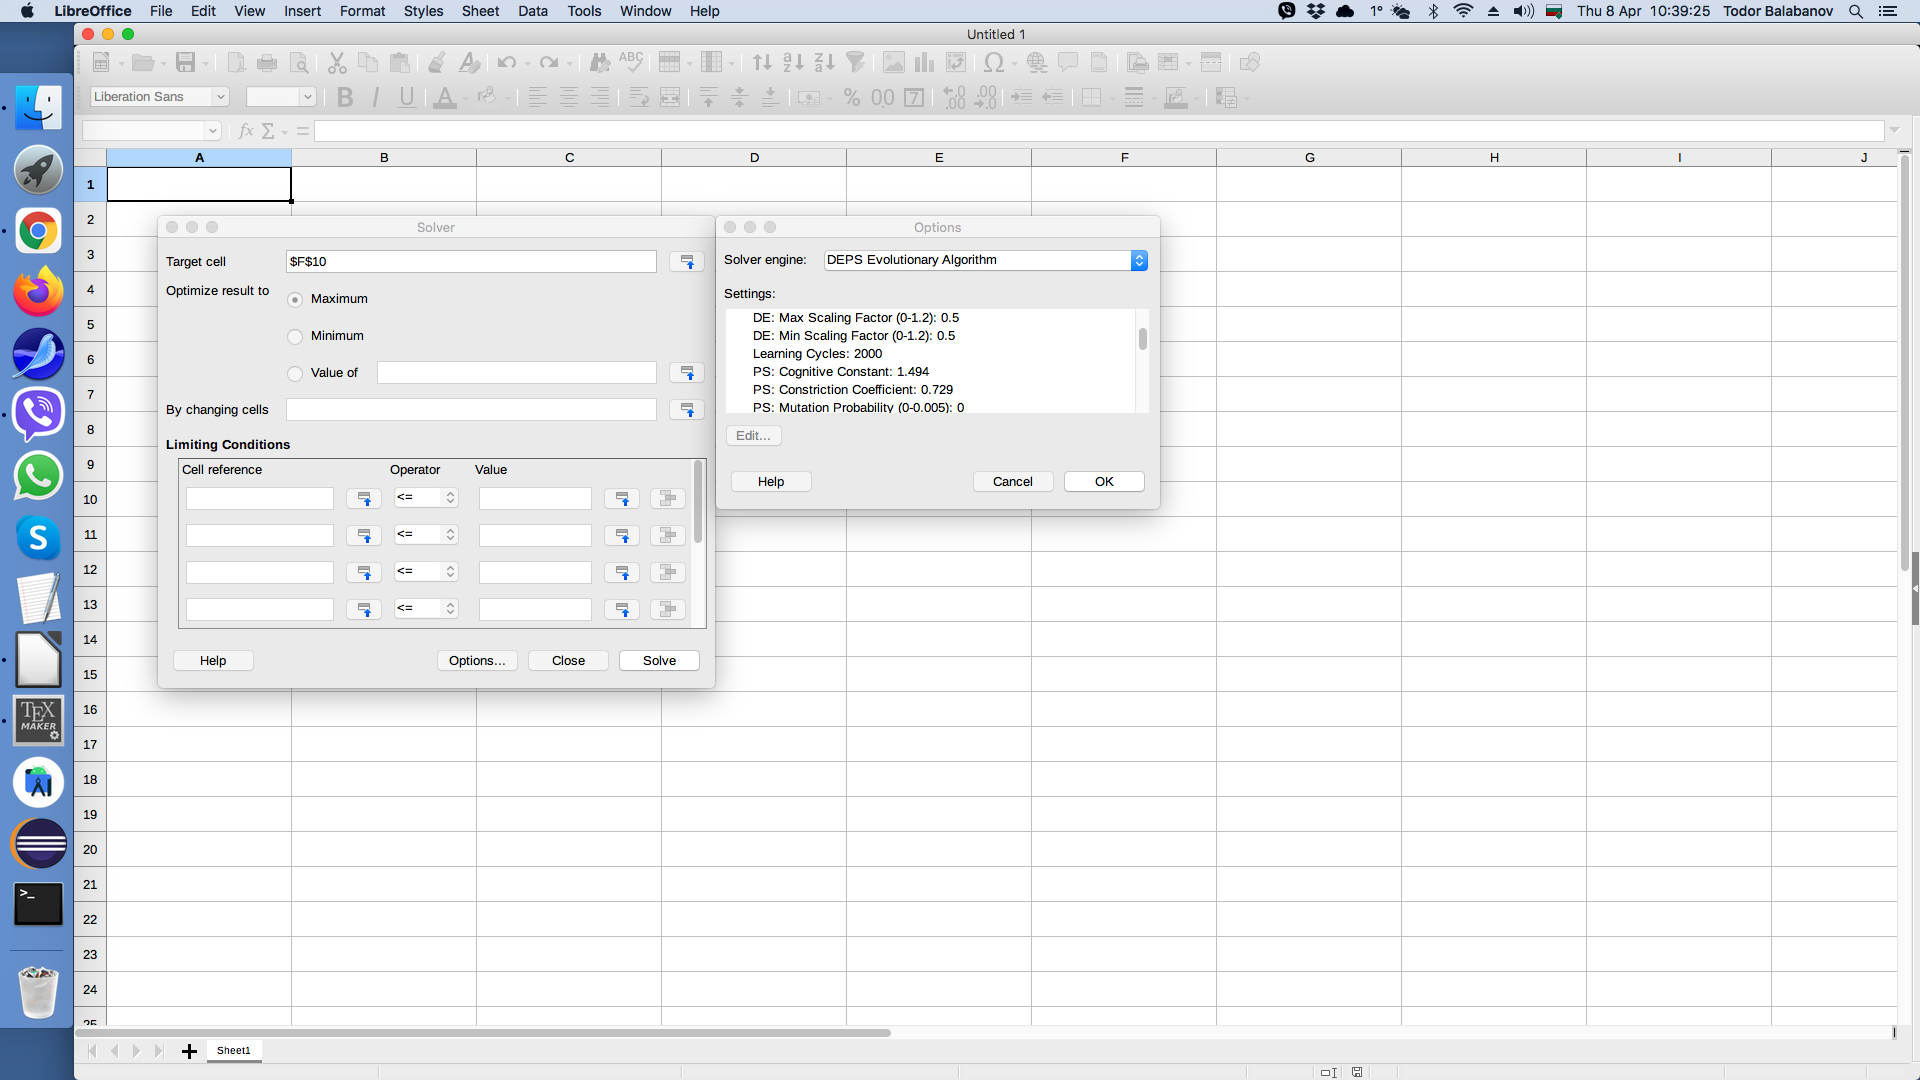
\includegraphics[width=1.0\linewidth]{fig001.png}
  \caption{Модул за оптимизация в LibreOffice Calc}
\label{fig001}
\end{figure}

За нелинейна оптимизация модулът прилага алгоритмите за еволюция на разликите и оптимизация с рояк от частици. Двата алгоритъма се прилагат в хибридна комбинация, като с предварително дефинирана вероятност е определено колко често ще бъде активиран всеки от тях. Модулът се настройва за клетка, чиято оптимална стойност ще бъде търсена (максимум, минимум или конкретно число). Също така, задава се и регионът от клетки, които подлежат на промяна в процеса по оптимизация. Като клетка в която ще се търси минимум при бързото протитипиране се избира общата средно-квадратична грешка допусната от изкуствената невронна мрежа. Регионът от клетки за оптимизация съдържа теглата използевани в изкуствената невронна мрежа. 

\begin{figure}[h]
  \centering
  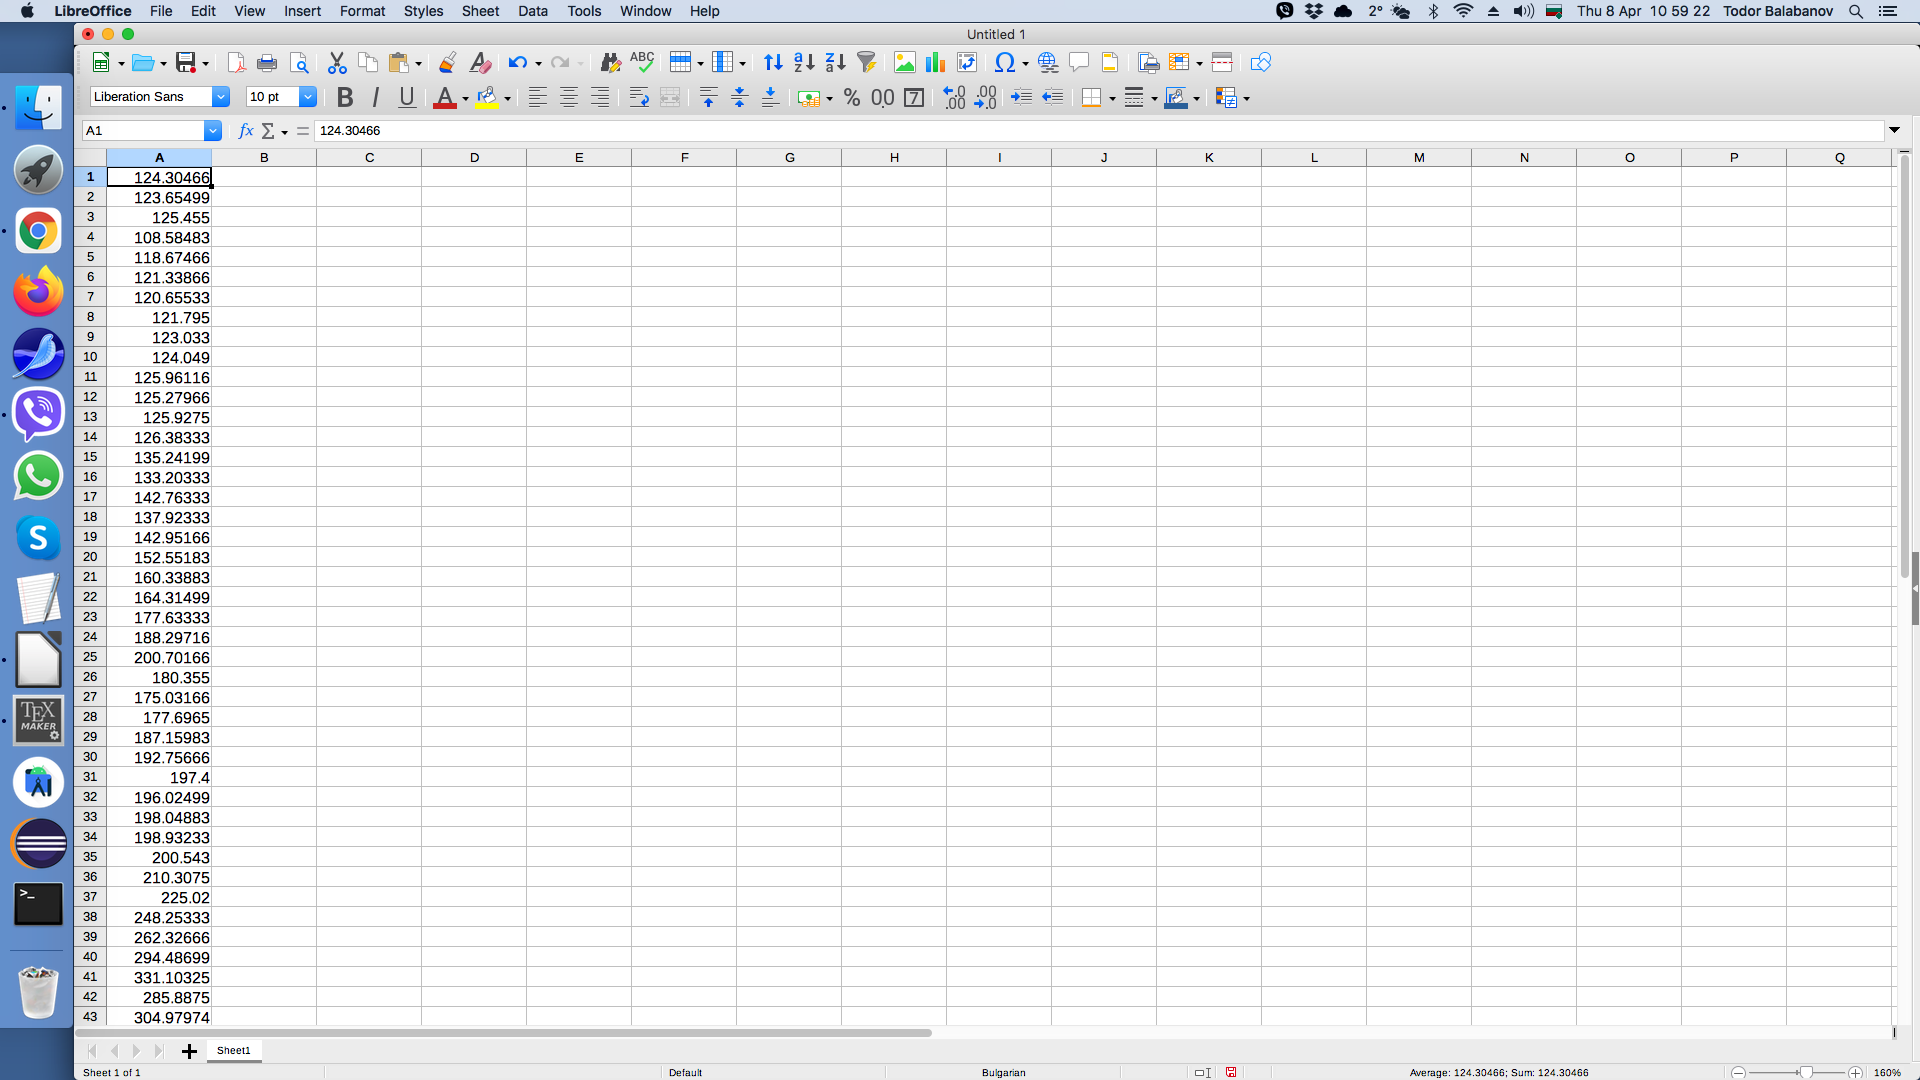
\includegraphics[width=1.0\linewidth]{fig002.png}
  \caption{Стойности на Bitcoin виртуалната валута}
\label{fig002}
\end{figure}

Като множество данни се използват стойностите на Bitcoin виртуалната валута (Фиг. \ref{fig002}), на дневна база, за няколко години назад. Моделът за прогнозиране се основава на нелинейна авторегресия. Това означава, че на входа на мрежата се подават мащабирани минали стойности от времевия ред, а на изхода на мрежата се очакват мащабирани прогнозни стойности. 

\begin{figure}[h]
  \centering
  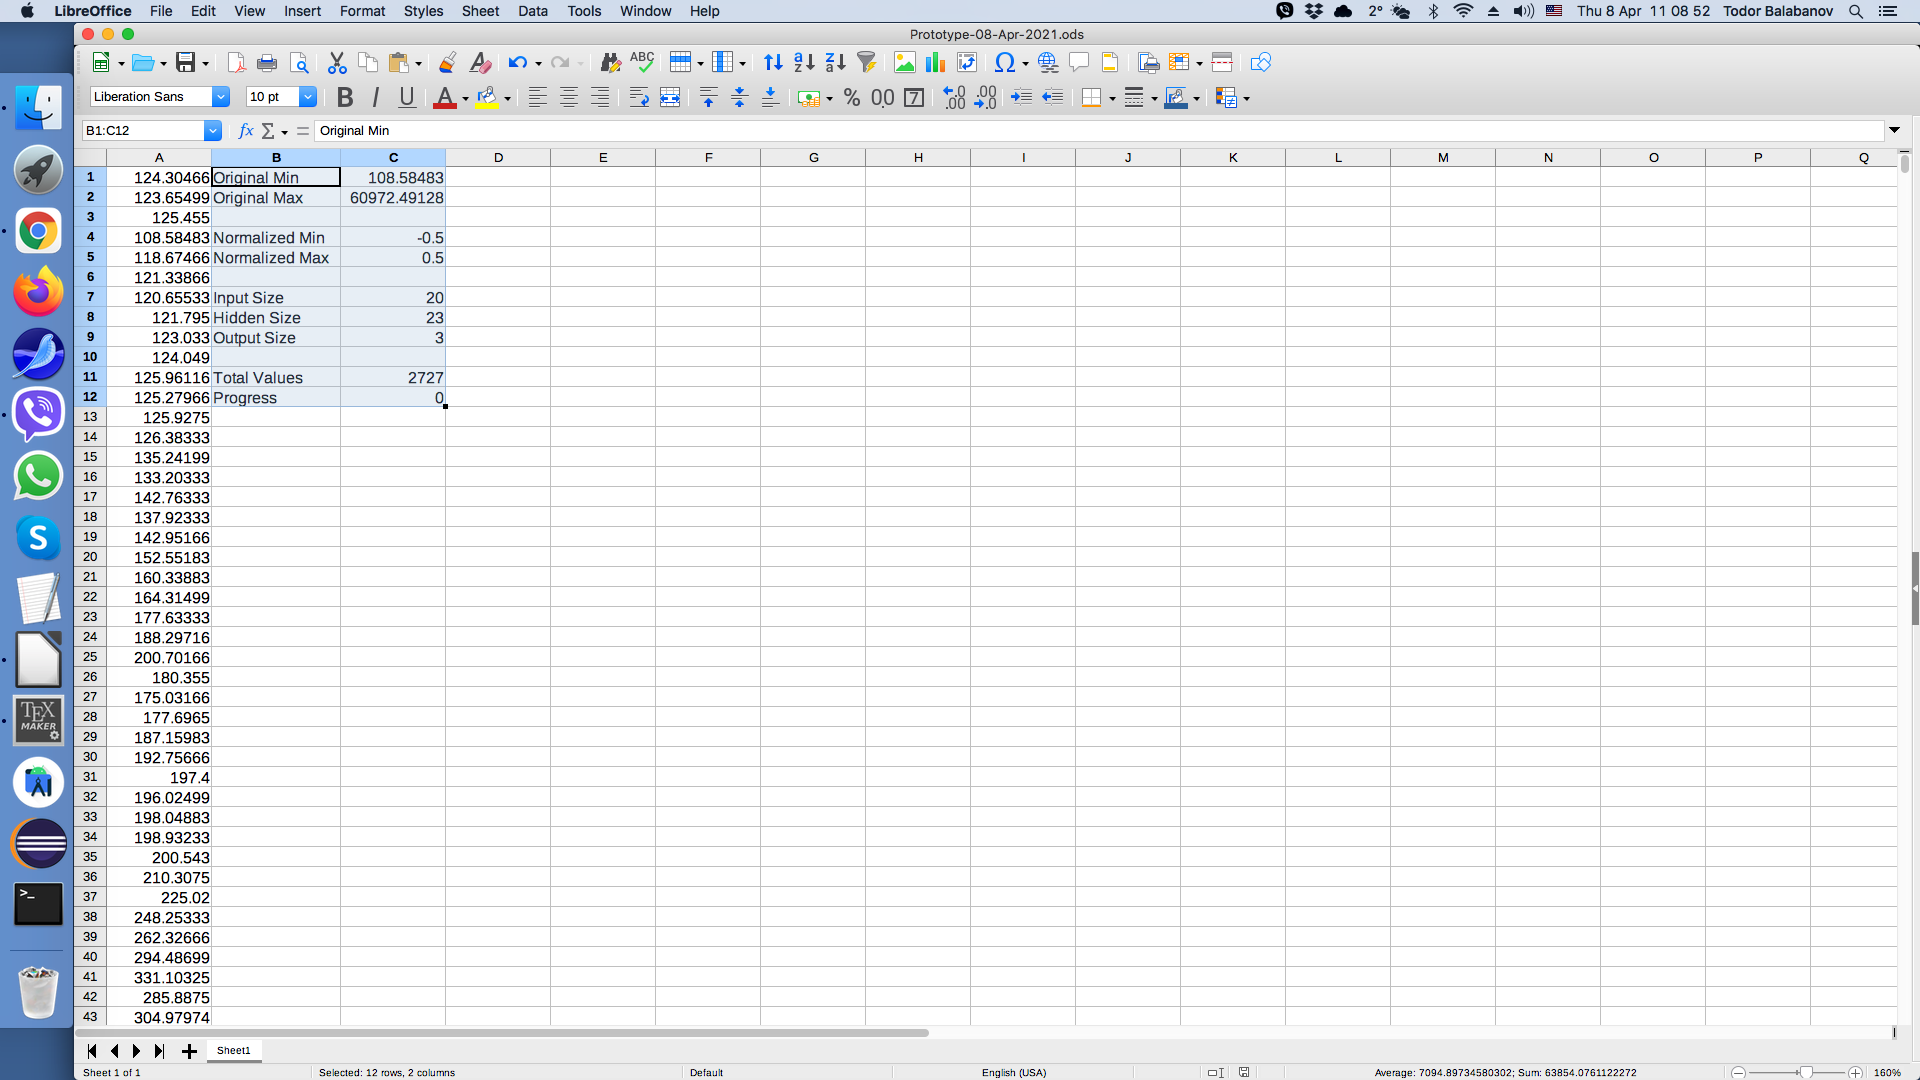
\includegraphics[width=1.0\linewidth]{fig003.png}
  \caption{Параметри на трислойната изкуствена невронна мрежа}
\label{fig003}
\end{figure}

След подбора на времеви ред следва избор на параметрите с които ще бъде напревен модела на трислойната изкуствена невронна мрежа (Фиг. \ref{fig003}). За целите на линейното мащабиране първо се намират най-малката и най-голямата стойност в оригиналния времеви ред, чрез формули в LibreOffice Calc: $=MIN(A:A)$ и $=MAX(A:A)$. Тъй като приложената прагова функция е хиперболичен тангенс, диапазона за мащабирания времеви ред е избран от -0.5 до +0.5. Умишлено се избягва мащабиране до асимптотичните стойности от -1.0 до +1.0, тъй като такова мащабиране много би увеличило стойностите на междинните пресмятания, а и не би дало възможност да се прогнозират по-малки или по-големи стойности от вече известните в оригиналния времеви ред. Топологията на мрежата се избира експериментално, като изходния слой има размер, според това колко стойности в бъдещето е желателно да се предсказват. Размера на входния слой се определя експериментално. За размера на скрития слой има различни емпирични правила, като най-популярното е скритият слой да бъде половината от сумата на размерите имащи входния и изходния слой. Съществуват адаптивни алгоритми, които чрез проби и грешки да определят топологията на мрежата, но в това бързо прототипиране тези алгоритми не се прилагат. 

Общият брой стойности в оригиналния времеви ред се определят с формула в LibreOffice Calc: $=COUNT(A:A)$. Тъй като процеса по „разгръщането“ на модела е относително бавен, то се добавя клетка в която да се проследява напредъка от Python скрипта в „разгръщането“. LibreOffice Calc позволява изпълнението на макроси, като се поддържат няколко програмни езика. Програмният език Python е изключително популярен в сферата на машинното самообучение и дава изключително големи възможности за частична автоматизация в програмите на LibreOffice.

След мащабирането на оригиналния времеви ред се формират тренировъчните примери, като за вход се вземат стойности преди условния момент $t_0$, а за очакван изход стойности след условния момент $t_0$ (условно разделяне на минало и бъдеще).

\begin{lstlisting}[caption=Мащабиране на оригиналния времеви ред, language=Python, basicstyle=\tiny, label=listing001]
    ''' Scale input. '''
    for t in range(1, total_values + 1):
        sheet.getCellRangeByName("E" + str(t)).setValue(sheet.getCellRangeByName("$C$4").getValue() + 
        (sheet.getCellRangeByName("$C$5").getValue() - sheet.getCellRangeByName("$C$4").getValue()) * ((sheet.getCellRangeByName("A" + str(t)).getValue() - 
        sheet.getCellRangeByName("$C$1").getValue()) / (sheet.getCellRangeByName("$C$2").getValue() - sheet.getCellRangeByName("$C$1").getValue())))
\end{lstlisting}

В листинг \ref{listing001} се демонстрира линейното мащабиране, като за извършване на изчисленията се използват установените минимални и максимални стойности (Фиг. \ref{fig004}). 

\begin{figure}[h]
  \centering
  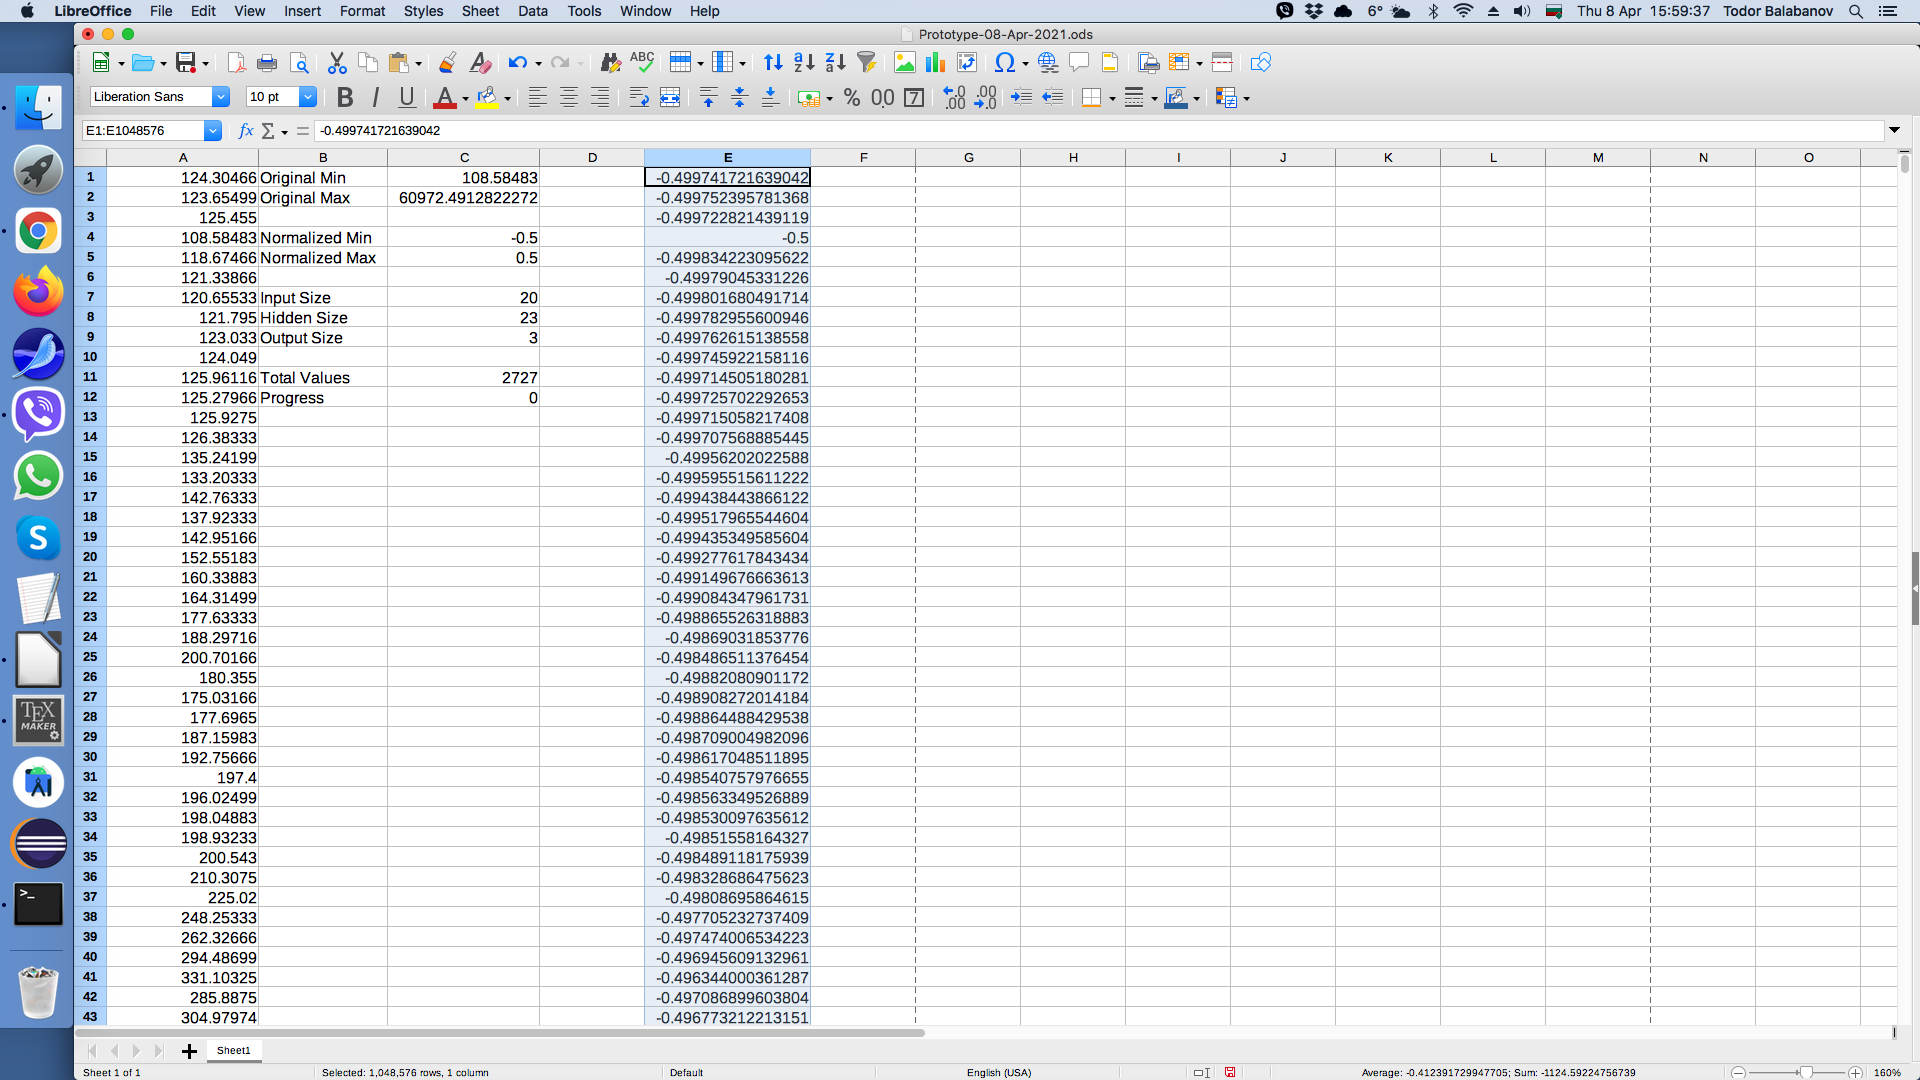
\includegraphics[width=1.0\linewidth]{fig004.png}
  \caption{Резултат от мащабирането на времевия ред}
\label{fig004}
\end{figure}

На всеки слой в изкуствената невронна мрежа се добавя по един допълнителен неврон (Листинг \ref{listing002}), постоянно емитиращ единична стойност (отместване или от английски език bias).

\begin{lstlisting}[caption=Неврони емитиращи постоянно единичен сигнал, language=Python, basicstyle=\tiny, label=listing002]
        ''' Setup biases. '''
        sheet.getCellRangeByName("G" + str(x)).setValue(1)
        sheet.getCellRangeByName("G" + str(x)).CellBackColor = (255 << 16 | 255 << 8 | 0)
        sheet.getCellRangeByName("H" + str(x)).setValue(1)
        sheet.getCellRangeByName("H" + str(x)).CellBackColor = (255 << 16 | 255 << 8 | 0)
        sheet.getCellRangeByName("I" + str(x)).setValue(1)
        sheet.getCellRangeByName("I" + str(x)).CellBackColor = (255 << 16 | 255 << 8 | 0)
        sheet.getCellRangeByName("J" + str(x)).setValue(1)
        sheet.getCellRangeByName("J" + str(x)).CellBackColor = (255 << 16 | 255 << 8 | 0)
\end{lstlisting}

Мащабираният времеви ред бива „разбит“ условно на „минали“ стойности и „бъдещи“ стойности. Миналите стойности стават входни сигнали за изкуствената невронна мрежа (Листинг \ref{listing003}).

\begin{lstlisting}[caption=Формиране на входния слой, language=Python, basicstyle=\tiny, label=listing003]
        ''' Input data loading. '''
        for i in range(1, input_size + 1):
            sheet.getCellRangeByName("G" + str(x + i)).setValue(sheet.getCellRangeByName("E" + str(t + i)).getValue())
            sheet.getCellRangeByName("G" + str(x + i)).CellBackColor = (255 << 16 | 0 << 8 | 0)
\end{lstlisting}

По аналогичен начин, будещите стойности се зареждат като очакван изход от изкуствената невронна мрежа (Листинг \ref{listing004}).

\begin{lstlisting}[caption=Очакван изход от мрежата, language=Python, basicstyle=\tiny, label=listing004]
        ''' Expected data loading. '''
        for e in range(1, output_size + 1):
            sheet.getCellRangeByName("J" + str(x + e)).setValue(sheet.getCellRangeByName("E" + str(t + e + input_size)).getValue())
            sheet.getCellRangeByName("J" + str(x + e)).CellBackColor = (0 << 16 | 127 << 8 | 0)
\end{lstlisting}

Стойностите във възлите на скрития слой са резултат от пресмятане на входните сигнали и текущите стойности на теглата в мрежата (Листинг \ref{listing005}). 

\begin{lstlisting}[caption=Стойности на скрития слой при правия пас, language=Python, basicstyle=\tiny, label=listing005]
        ''' Setup hidden layer. '''
        wih = 1
        for h in range(1, hidden_size + 1):
            sum = ""
            for i in range(0, input_size + 1):
                sum = sum + "G" + str(x + i) + "*Q" + str(wih)
                wih = wih + 1
                if i < input_size:
                    sum = sum + " + "
            sheet.getCellRangeByName("H" + str(x + h)).setFormula("=TANH( " + sum + " )")
            sheet.getCellRangeByName("H" + str(x + h)).CellBackColor = (0 << 16 | 0 << 8 | 255)
\end{lstlisting}

На свой ред, стойностите в изходния слой са резултат от пресмятане на сигналите в скрития слой и текущите стойности на теглата в мрежата (Листинг \ref{listing006}).

\begin{lstlisting}[caption=Стойности на изходния слой при правия пас, language=Python, basicstyle=\tiny, label=listing006]
        ''' Setup output layer. '''
        who = 1
        for o in range(1, output_size + 1):
            sum = ""
            for h in range(0, hidden_size + 1):
                sum = sum + "H" + str(x + h) + "*S" + str(who)
                who = who + 1
                if h < hidden_size:
                    sum = sum + " + "
            sheet.getCellRangeByName("I" + str(x + o)).setFormula("=TANH( " + sum + " )")
            sheet.getCellRangeByName("I" + str(x + o)).CellBackColor = (0 << 16 | 255 << 8 | 0)
\end{lstlisting}

Стойностите в изходния слой, спрямо очакваните стойности дават грешката, която изкуствената невронна мрежа допуска за конкретния тренировъчен пример (Листинг \ref{listing007}).

\begin{lstlisting}[caption=Стойност на грешката допусната от мрежата за конкретния пример, language=Python, basicstyle=\tiny, label=listing007]
        ''' Network output error. '''
        for r in range(1, output_size + 1):
            sheet.getCellRangeByName("K" + str(x + r)).setFormula("= (J" + str(x + r) + "-I" + str(x + r) + ") * (J" + str(x + r) + "-I" + str(x + r) + ")")
            sheet.getCellRangeByName("K" + str(x + r)).CellBackColor = (0 << 16 | 255 << 8 | 255)
\end{lstlisting}

Така описаното разполагане по клетките на листа в електронната таблица се повтаря многократно, така че да се появи фрагмент за всеки тренировъчен пример. Фрагментът съдържа входен слой, скрит слой, изходен слой и очаквани на изхода стойности (Фиг. \ref{fig005}).

\begin{figure}[h]
  \centering
  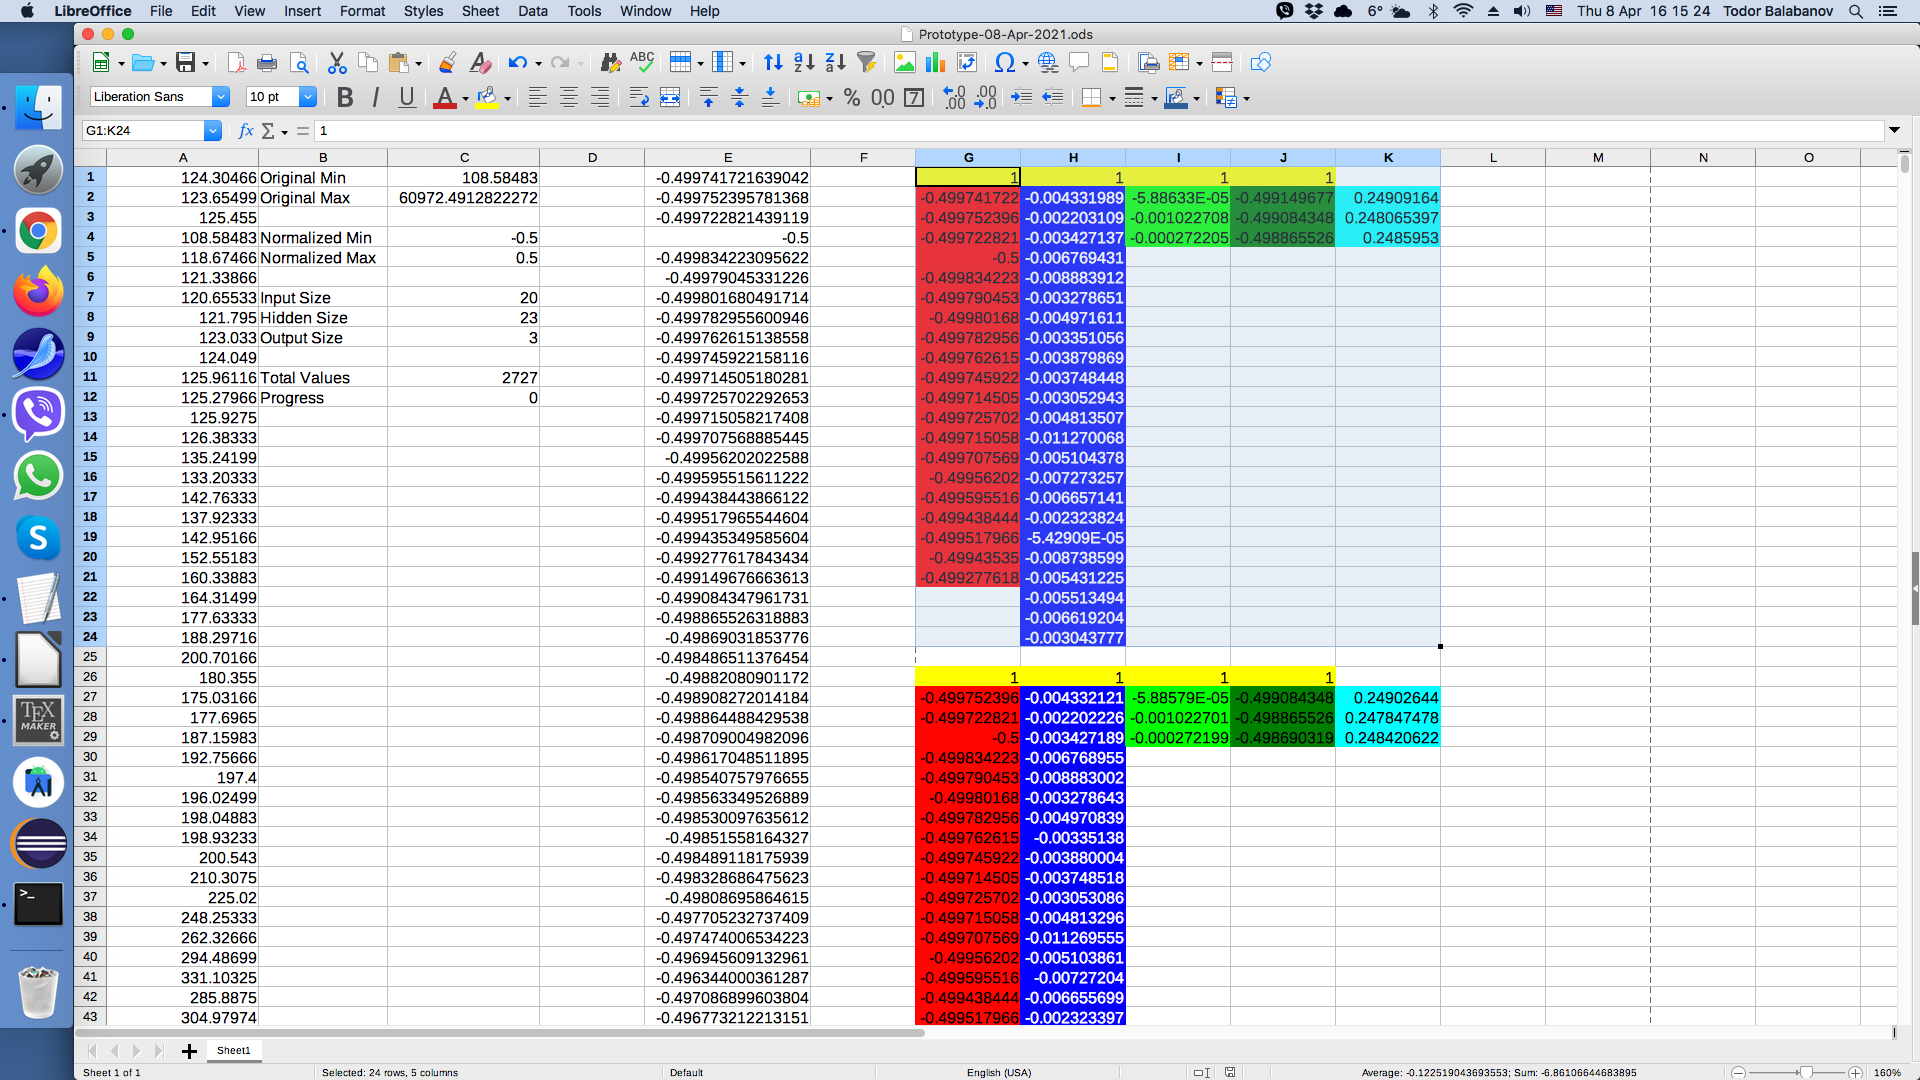
\includegraphics[width=1.0\linewidth]{fig005.png}
  \caption{Фрагменти за тренировъчните примери}
\label{fig005}
\end{figure}

Общата грешка, допусната от мрежата при всички тренировъчни примери е на базата на средно-квадратична грешка (Листинг \ref{listing008}).

\begin{lstlisting}[caption=Обща средно-квадратична грешка на мрежата, language=Python, basicstyle=\tiny, label=listing008]
    ''' Network total error. '''
    sheet.getCellRangeByName("M1").setFormula("= SQRT( SUM(K:K) / COUNT(K:K) )")
    sheet.getCellRangeByName("M1").CellBackColor = 0
\end{lstlisting}

Два региона клетки в листа на електронната таблица се определят за стойностите на теглата в мрежата, както и обратно мащабиране към оригиналните стойности (Листинг \ref{listing009}).

\begin{lstlisting}[caption=Определяне на региони за теглата на мрежата, language=Python, basicstyle=\tiny, label=listing009]
    ''' Setup hidden layer weights. '''
    wih = 1
    for h in range(2, hidden_size + 2):
        for i in range(1, input_size + 2):
            sheet.getCellRangeByName("Q" + str(wih)).CellBackColor = (255 << 16 | 0 << 8 | 255)
            wih = wih + 1
        
    ''' Setup output layer weights. '''
    who = 1
    for o in range(2, output_size + 2):
        for h in range(1, hidden_size + 2):
            sheet.getCellRangeByName("S" + str(who)).CellBackColor = (255 << 16 | 0 << 8 | 255)
            who = who + 1

        sheet.getCellRangeByName("U" + str(o)).setFormula("=$C$1 + ($C$2 - $C$1) * ((T" + str(o) + " - $C$4) / ($C$5 - $C$4))")
        sheet.getCellRangeByName("U" + str(o)).CellBackColor = (0 << 16 | 127 << 8 | 0)
\end{lstlisting}

За да не се блокира графичния потребителски интерфейс, „разгръщането“ на модела на изкуствената невронна мрежа се извършва в отделна нишка (Листинг \ref{listing010}).


\begin{lstlisting}[caption=Изпълнение с отделна нишка, language=Python, basicstyle=\tiny, label=listing010]
def BuildAnnModel():
    thread = Thread(target=ThreadWorker, args=(XSCRIPTCONTEXT.getDesktop(),))
    thread.start()
\end{lstlisting}


\chapter{Глава 3 - }
\chapter{Глава 4 - }

% Заключение.
\addcontentsline{toc}{chapter}{Заключение}
\chapter*{Заключение}

\newpage
\section*{Резюме на получените резултати}

\subsection*{Научно-приложни резултати}

\subsection*{Приложни резултати}

\newpage
\section*{Насоки за бъдещи изследвания}

\newpage
\section*{Публикации по темата на дисертационния труд}

\newpage
\section*{Забелязани цитирания}

\newpage
\section*{Декларация за оригиналност на резултатите}

\vspace{1cm}

Декларирам, че дисертацията съдържа оригинални резултати, получени при проведени от мен, научни изследвания с подкрепата и съдействието на научния ми ръководител.

Резултатите, които са получени, описани и/или публикувани от други учени, са коректно и подробно цитирани в библиографията.

Настоящият дисертационен труд не е прилаган за придобиване на научна степен в друго висше училище, университет или научен институт.

\vspace{2cm}

\begin{tabular}{ c c c c }
Дата: & .......................................... & Подпис: & .......................................... \\ 
& гр. София & & / Петър Томов / \\  
\end{tabular}


% Списък с използвана литература и източници на информация.
\addcontentsline{toc}{chapter}{Библиография}
%\chapter*{Библиография}

\begin{thebibliography}{99.}

\bibitem{Alba-01} Alba, E., Tomassini, M.: Parallelism and evolutionary algorithms. IEEE Transactions on Evolutionary Computation, vol. 6, no. 5, 443--462, 2002. ISSN 1089-778X DOI 10.1109/TEVC.2002.800880

\bibitem{Basheer-01} Basheer, I., Hajmeer, M.: Artificial neural networks: fundamentals, computing, design, and application. Journal of Microbiological Methods, vol. 43, no. 1, 3--31, 2000. ISSN 0167-7012 DOI 10.1016/S0167-7012(00)00201-3

\bibitem{Beyer-02} Beyer, H.: Evolutionary algorithms in noisy environments: theoretical issues and guidelines for practice. Computer Methods in Applied Mechanics and Engineering, vol. 186, no. 2-4, 239--267, 2000. ISSN 0045-7825 DOI 10.1016/S0045-7825(99)00386-2

\bibitem{Beyer-01} Beyer, H., Schwefel, H., Wegener, I.: How to analyse evolutionary algorithms. Theoretical Computer Science, vol. 287, no. 1, 101--130, 2002. ISSN 0304-3975 DOI 10.1016/S0304-3975(02)00137-8

\bibitem{Bilbao-01} Bilbao, I., Bilbao, J.: Overfitting problem and the over-training in the era of data: Particularly for Artificial Neural Networks. Proceedings of Eighth International Conference on Intelligent Computing and Information Systems, 173--177, 2017. ISBN 978-1-5386-0822-7 DOI 10.1109/INTELCIS.2017.8260032

\bibitem{Bing-01} Bing, Y., Hao, J., Zhang, S.: Stock Market Prediction Using Artificial Neural Networks. Advanced Engineering Forum, vol. 6-7, 1055--1060, 2012. ISSN 2234-991X DOI 10.4028/www.scientific.net/AEF.6-7.1055

\bibitem{Bontempi-01} Bontempi, G., Ben Taieb, S., Le Borgne Y.: Machine Learning Strategies for Time Series Forecasting. Lecture Notes in Business Information Processing, vol 138, 62--77, 2013. ISBN 978-3-642-36317-7 DOI 10.1007/978-3-642-36318-4\_3

\bibitem{Cao-01} Cao, L., Tay, F.: Support vector machine with adaptive parameters in financial time series forecasting. IEEE Transactions on Neural Networks, vol. 14, no. 6, 1506--1518, 2003. ISSN 1045-9227 DOI 10.1109/TNN.2003.820556

\bibitem{Cao-02} Cao, J., Li, Z., Li, J.: Financial time series forecasting model based on CEEMDAN and LSTM. Physica A: Statistical Mechanics and its Applications, vol. 519, 127--139, 2019. ISSN 0378-4371 DOI 10.1016/j.physa.2018.11.061

\bibitem{Caponetto-01} Caponetto, R., Fortuna, L., Fazzino, S., Xibilia, M.: Chaotic sequences to improve the performance of evolutionary algorithms. IEEE Transactions on Evolutionary Computation, vol. 7, no. 3, 289--304, 2003. DOI 10.1109/TEVC.2003.810069

\bibitem{Chandwani-01} Chandwani, V., Agrawal, V., Nagar, R.: Modeling slump of ready mix concrete using genetic algorithms assisted training of Artificial Neural Networks. Expert Systems with Applications, vol. 42, no. 2, 885--893, 2015. ISSN 0957-4174 DOI 10.1016/j.eswa.2014.08.048

\bibitem{Chen-01} Chen, Y., Yang, B., Dong, J., Abraham. A.: Time-series forecasting using flexible neural tree model. Information Sciences, vol. 174, no. 3--4, 219--235, 2005. ISSN 0020-0255 DOI 10.1016/j.ins.2004.10.005

\bibitem{Chen-02} Chen, J., Do, Q., Hsieh, H.: Training Artificial Neural Networks by a Hybrid PSO-CS Algorithm. Algorithms, vol. 8, no. 2, 292--308, 2015. ISSN 1999-4893 DOI 10.3390/a8020292

\bibitem{Cheng-01} Cheng, R., He, C., Jin, Y., Yao, X.: Model-based evolutionary algorithms: a short survey. Complex \& Intelligent Systems, vol. 4, 283--292, 2018. ISSN 2198-6053 DOI 10.1007/s40747-018-0080-1

\bibitem{Coello-01} Coello, C.: Theoretical and numerical constraint-handling techniques used with evolutionary algorithms: a survey of the state of the art. Computer Methods in Applied Mechanics and Engineering, vol. 191, no. 11-12, 1245--1287, 2002. ISSN 0045-7825 DOI 10.1016/S0045-7825(01)00323-1

\bibitem{Coello-02} Coello, C.: An Introduction to Evolutionary Algorithms and Their Applications. Proceedings of International Symposium and School on Advanced Distributed Systems, vol. 3563, 425--442, 2005. ISBN 978-3-540-28063-7 DOI 10.1007/11533962\_39

\bibitem{Cortez-01} Cortez, P., Rocha, M., Neves, J.: Evolving Time Series Forecasting ARMA Models. Journal of Heuristics, vol. 10, no. 4, 415--429, 2004. ISSN 1381-1231 DOI 10.1023/B:HEUR.0000034714.09838.1e

\bibitem{Coulibaly-01} Coulibaly, P., Anctil, F., Bobee, B.: Daily reservoir inflow forecasting using artificial neural networks with stopped training approach. Journal of Hydrology, vol. 230, no. 3-4, 244--257, 2000. ISSN 0022-1694 DOI 10.1016/S0022-1694(00)00214-6

\bibitem{Cui-01} Cui, Z., Yang, C., Sanyal, S.: Training artificial neural networks using APPM. International Journal of Wireless and Mobile Computing, vol. 5, no. 2, 168--174, 2012. ISSN 1741-1084 DOI 10.1504/IJWMC.2012.046787

\bibitem{da-Silva-01} da Silva, I., Hernane Spatti, D., Andrade Flauzino, R., Liboni, L., dos Reis Alves, S.: Artificial Neural Network Architectures and Training Processes. Artificial Neural Networks, 21--28, 2017. ISBN 978-3-319-43161-1 DOI 10.1007/978-3-319-43162-8\_2

\bibitem{Ding-01} Ding, S., Li, H., Su, C., Yu, J., Jin, F.: Evolutionary artificial neural networks: a review. Artificial Intelligence Review, vol. 39, no. 3, 251--260, 2013. ISSN 0269-2821 DOI 10.1007/s10462-011-9270-6

\bibitem{Diosan-01} Diosan, L., Oltean, M.: Evolutionary design of Evolutionary Algorithms. Genetic Programming and Evolvable Machines, vol. 10, 263--306, 2009. ISSN 1389-2576 DOI 10.1007/s10710-009-9081-6

\bibitem{Eiben-01} Eiben, A., Michalewicz, Z., Schoenauer, M., Smith, J.: Parameter Control in Evolutionary Algorithms. Parameter Setting in Evolutionary Algorithms, vol. 54, 19--46, 2007. ISBN 978-3-540-69431-1 DOI 10.1007/978-3-540-69432-8\_2

\bibitem{Eiben-02} Eiben, A., Smit, S.: Parameter tuning for configuring and analyzing evolutionary algorithms. Swarm and Evolutionary Computation, vol. 1, no. 1, 19--31, 2011. ISSN 2210-6502 DOI 10.1016/j.swevo.2011.02.001

\bibitem{El-Abd-01} El-Abd, M.: Performance assessment of foraging algorithms vs. evolutionary algorithms. Information Sciences, vol. 182, no. 1, 243--263, 2012. ISSN 0020-0255 DOI 10.1016/j.ins.2011.09.005

\bibitem{Ertugrul-01} Ertugrul, O.: A novel type of activation function in artificial neural networks: Trained activation function. Neural Networks, vol. 99, 148--157, 2018. ISSN 0893-6080 DOI 10.1016/j.neunet.2018.01.007

\bibitem{Francois-01} Francois, O., Lavergne, C.: Design of evolutionary algorithms-A statistical perspective. IEEE Transactions on Evolutionary Computation, vol. 5, no. 2, 129--148, 2001. ISSN 1089-778X DOI 10.1109/4235.918434

\bibitem{Gooijer-01} Gooijer, J., Hyndman, R.: 25 years of time series forecasting. International Journal of Forecasting, vol. 22, no. 3, 443--473, 2006. ISSN 0169-2070 DOI 10.1016/j.ijforecast.2006.01.001

\bibitem{Grosan-01} Grosan, C., Abraham, A.: Hybrid Evolutionary Algorithms: Methodologies, Architectures, and Reviews. Hybrid Evolutionary Algorithms, vol 75, 1--17, 2007. ISBN 978-3-540-73296-9 DOI 10.1007/978-3-540-73297-6\_1

\bibitem{Hamzacebi-01} Hamzacebi, C.: Improving artificial neural networks’ performance in seasonal time series forecasting. Information Sciences, vol. 178, no. 23, 4550--4559, 2008. ISSN 0020-0255 DOI 10.1016/j.ins.2008.07.024

\bibitem{He-02} He, J., Yu, X.: Conditions for the convergence of evolutionary algorithms. Journal of Systems Architecture, vol. 47, no. 7, 601--612, 2001. ISSN 1383-7621 DOI 10.1016/S1383-7621(01)00018-2

\bibitem{He-01} He, J., Yao, X.: Towards an analytic framework for analysing the computation time of evolutionary algorithms. Artificial Intelligence, vol. 145, no. 1-2, 59--97, 2003. ISSN 0004-3702 DOI 10.1016/S0004-3702(02)00381-8

\bibitem{Jain-02} Jain, A., Mao, J., Mohiuddin, K.: Artificial neural networks: a tutorial. Computer, vol. 29, no. 3, 31--44, 1996. ISSN 0018-9162 DOI 10.1109/2.485891

\bibitem{Jain-01} Jain, A., Kumar, A.: Hybrid neural network models for hydrologic time series forecasting. Applied Soft Computing, vol. 7, no. 2, 585--592, 2007. ISSN 1568-4946 DOI 10.1016/j.asoc.2006.03.002

\bibitem{Joo-01} Joo, T., Kim, S.: Time series forecasting based on wavelet filtering. Expert Systems with Applications, vol. 42, no. 8, 3868--3874, 2015. ISSN 0957-4174 DOI 10.1016/j.eswa.2015.01.026

\bibitem{Kachitvichyanukul-01} Kachitvichyanukul, V.: Comparison of Three Evolutionary Algorithms: GA, PSO, and DE. Industrial Engineering and Management Systems, vol. 11, no. 3, 215--223, 2012. ISSN 1598-7248 DOI 10.7232/iems.2012.11.3.215

\bibitem{Karaboga-01} Karaboga, D., Akay, B., Ozturk, C.: Artificial Bee Colony (ABC) Optimization Algorithm for Training Feed-Forward Neural Networks. Proceedings of International Conference on Modeling Decisions for Artificial Intelligence, vol. 4617, 318--329, 2007. ISBN 978-3-540-73728-5 DOI 10.1007/978-3-540-73729-2\_30

\bibitem{Karafotias-01} Karafotias, G., Hoogendoorn, M., Eiben, A.: Parameter Control in Evolutionary Algorithms: Trends and Challenges. IEEE Transactions on Evolutionary Computation, vol. 19, no. 2, 167--187, 2015. ISSN 1089-778X DOI 10.1109/TEVC.2014.2308294

\bibitem{Karnin-01} Karnin, E.: A simple procedure for pruning back-propagation trained neural networks. IEEE Transactions on Neural Networks, vol. 1, no. 2, 239--242, 1990. ISSN 1045-9227 DOI 10.1109/72.80236

\bibitem{Kattan-01} Kattan, A., Abdullah, R., Salam, R.: Harmony Search Based Supervised Training of Artificial Neural Networks. Proceedings of International Conference on Intelligent Systems, Modelling and Simulation, 105--110, 2010. ISBN 978-1-4244-5984-1 DOI 10.1109/ISMS.2010.31

\bibitem{Kazimipour-01} Kazimipour, B., Li, X., Qin, A.: A review of population initialization techniques for evolutionary algorithms. Proceedings of IEEE Congress on Evolutionary Computation, 2585--2592, 2014. ISBN 978-1-4799-1488-3 DOI 10.1109/CEC.2014.6900618

\bibitem{Kern-01} Kern, S., Muller, S., Hansen, N., Buche, D., Ocenasek, J., Koumoutsakos, P.: Learning probability distributions in continuous evolutionary algorithms - a comparative review. Natural Computing, vol. 3, 77--112, 2004. ISSN 1572-9796 DOI 10.1023/B:NACO.0000023416.59689.4e

\bibitem{Khashei-01} Khashei, M., Bijari, M.: An artificial neural network (p,d,q) model for timeseries forecasting. Expert Systems with Applications, vol. 37, no. 1, 479--489, 2010. ISSN 0957-4174 DOI 10.1016/j.eswa.2009.05.044

\bibitem{Khashei-03} Khashei, M., Bijari, M.: A novel hybridization of artificial neural networks and ARIMA models for time series forecasting. Applied Soft Computing, vol. 11, no. 2, 2664--2675, 2011. ISSN 1568-4946 DOI 10.1016/j.asoc.2010.10.015

\bibitem{Khashei-02} Khashei, M., Bijari. M.: A new class of hybrid models for time series forecasting. Expert Systems with Applications, vol. 39, no. 4, 4344-4357, 2012. ISSN 0957-4174 DOI 10.1016/j.eswa.2011.09.157

\bibitem{Kingston-01} Kingston, G., Lambert, M., Maier, H.: Bayesian training of artificial neural networks used for water resources modeling. Water Resources Research, vol. 41, no. 12, W12409, 2005. ISSN 0043-1397 DOI 10.1029/2005WR004152

\bibitem{Kollias-01} Kollias, S., Anastassiou, D.: An adaptive least squares algorithm for the efficient training of artificial neural networks. IEEE Transactions on Circuits and Systems, vol. 36, no. 8, 1092--1101, 1989. ISSN 0098-4094 DOI 10.1109/31.192419

\bibitem{Koziel-01} Koziel, S., Michalewicz, Z.: Evolutionary Algorithms, Homomorphous Mappings, and Constrained Parameter Optimization. Evolutionary Computation, vol. 7, no. 1, 19--44, 1999. ISSN 1063-6560 DOI 10.1162/evco.1999.7.1.19.

\bibitem{Kubat-01} Kubat, M.: Artificial Neural Networks. An Introduction to Machine Learning, 91--111, 2015. ISBN 978-3-319-20009-5 DOI 10.1007/978-3-319-20010-1\_5

\bibitem{Kyoung-jae-01} Kyoung-jae, K.: Financial time series forecasting using support vector machines. Neurocomputing, vol. 55, no. 1, 307--319, 2003. ISSN 0925-2312 DOI 10.1016/S0925-2312(03)00372-2

\bibitem{Lachtermacher-01} Lachtermacher, G., Fuller, J: Back propagation in time-series forecasting. Journal of Forecasting, vol. 14, no. 4, 381--393, 1995. ISSN 1099-131X DOI 10.1002/for.3980140405

\bibitem{Lagaros-01} Lagaros, N., Papadrakakis, M., Kokossalakis, G.: Structural optimization using evolutionary algorithms. Computers \& Structures, vol. 80, no. 7-8, 571--589, 2002. ISSN 0045-7949 DOI S0045-7949(02)00027-5

\bibitem{Lu-01} Lu, C., Lee, T., Chiu. C.: Financial time series forecasting using independent component analysis and support vector regression. Decision Support Systems, vol. 47, no. 2, 115--125, 2009. ISSN 0167-9236 DOI 10.1016/j.dss.2009.02.001

\bibitem{Mocanu-01} Mocanu, D., Mocanu, E., Stone, P., Nguyen, P., Gibescu, M., Liotta, A.: Scalable training of artificial neural networks with adaptive sparse connectivity inspired by network science. Nature Communications, vol. 9, 2383, 2018. ISSN 2041-1723 DOI 10.1038/s41467-018-04316-3

\bibitem{Naudts-01} Naudts, B., Kallel, L.: A comparison of predictive measures of problem difficulty in evolutionary algorithms. IEEE Transactions on Evolutionary Computation, vol. 4, no. 1, 1--15, 2000. ISSN 1089-778X DOI 10.1109/4235.843491

\bibitem{Nawi-01} Nawi, N., Atomi, W., Rehman, M.: The Effect of Data Pre-processing on Optimized Training of Artificial Neural Networks. Procedia Technology, vol. 11, 32--39, 2013. ISSN 2212-0173 DOI 10.1016/j.protcy.2013.12.159

\bibitem{Nelson-01} Nelson, M., Hill, T., Remus, W., O'Connor, M.: Time series forecasting using neural networks: should the data be deseasonalized first?. Journal of Forecasting, vol. 18, no. 5, 359--367, 1999. ISSN 1099-131X DOI 10.1002/(SICI)1099-131X(199909)18:5<359::AID-FOR746>3.0.CO;2-P

\bibitem{Oliveira-01} Oliveira, M., Torgo, L.: Ensembles for Time Series Forecasting. Proceedings of the Sixth Asian Conference on Machine Learning, vol. 39, 360--370, 2015. ISSN 2640-3498

\bibitem{Piotrowski-01} Piotrowski, A., Osuch, M., Napiorkowski, M., Rowinski, P., Napiorkowski, J.: Comparing large number of metaheuristics for artificial neural networks training to predict water temperature in a natural river. Computers \& Geosciences, vol. 64, 136--151, 2014. ISSN 0098-3004 DOI 10.1016/j.cageo.2013.12.013

\bibitem{Pomerleau-01} Pomerleau, D: Efficient Training of Artificial Neural Networks for Autonomous Navigation. Neural Computation, vol. 3, no. 1, 88--97, 1991. ISSN 0899-7667 DOI 10.1162/neco.1991.3.1.88

\bibitem{Pradhan-01} Pradhan, B., Naghibi, S., Motevalli, A., Mansor, S: Assessment of the effects of training data selection on the landslide susceptibility mapping: a comparison between support vector machine (SVM), logistic regression (LR) and artificial neural networks (ANN). Geomatics, Natural Hazards and Risk, vol. 9, no. 1, 49--69, 2018. ISSN 1947-5705 DOI 10.1080/19475705.2017.1407368

\bibitem{Qi-01} Qi, M., Zhang, G.: An investigation of model selection criteria for neural network time series forecasting. European Journal of Operational Research, vol. 132, no. 3, 666--680, 2001. ISSN 0377-2217 DOI 10.1016/S0377-2217(00)00171-5

\bibitem{Roy-01} Roy, A., Dutta, D., Choudhury, K.: Training Artificial Neural Network using Particle Swarm Optimization Algorithm. International Journal of Advanced Research in Computer Science and Software Engineering, vol. 3, no. 3, 430--434, ISSN 2277-128X

\bibitem{Ryerkerk-01} Ryerkerk, M., Averill, R., Deb, K., Goodman, Е.: A survey of evolutionary algorithms using metameric representations. Genetic Programming and Evolvable Machines, vol. 20, 441--478, 2019. ISSN 1389-2576 DOI 10.1007/s10710-019-09356-2

\bibitem{Salami-01} Salami, M., Hendtlass, T.: A fast evaluation strategy for evolutionary algorithms. Applied Soft Computing, vol. 2, no. 3, 156--173, 2003. ISSN 1568-4946 DOI 10.1016/S1568-4946(02)00067-4

\bibitem{Sequin-01} Sequin, C., Clay, R.: Fault tolerance in artificial neural networks. Proceedings of International Joint Conference on Neural Networks, vol. 1, 703--708, 1990. DOI 10.1109/IJCNN.1990.137651

\bibitem{Shen-01} Shen, Z., Zhang, Y., Lu, J., Xu, J., Xiao, G.: A novel time series forecasting model with deep learning. Neurocomputing, vol. 396, 302--313, 2020. ISSN 0925-2312 DOI 10.1016/j.neucom.2018.12.084

\bibitem{Sietsma-01} Sietsma, J., Dow, R.: Creating artificial neural networks that generalize. Neural Networks, vol. 4, no. 1, 67--79, 1991. ISSN 0893-6080 DOI 10.1016/0893-6080(91)90033-2

\bibitem{Singh-01} Singh, S.: Pattern Modelling in Time-series Forecasting. Cybernetics and Systems, vol. 31, no. 1, 49--65, 2000. ISSN 0196-9722 DOI 10.1080/019697200124919

\bibitem{Slowik-01} Slowik, A., Bialko, M.: Training of artificial neural networks using differential evolution algorithm. Proceedings of Conference on Human System Interactions, 60--65, 2008. ISBN 978-1-4244-1542-7 DOI 10.1109/HSI.2008.4581409

\bibitem{Slowik-02} Slowik, A., Kwasnicka, H.: Evolutionary algorithms and their applications to engineering problems. Neural Computing and Applications vol. 32, 12363--12379, 2020. ISSN 0941-0643 DOI 10.1007/s00521-020-04832-8

\bibitem{Tang-01} Tang, Z., de Almeida, C., Fishwick, P.: Time series forecasting using neural networks vs Box-Jenkins methodology. SIMULATION, vol. 57, no. 5, 303-310, 1991. ISSN 0037-5497 DOI 10.1177/003754979105700508

\bibitem{Tay-01} Tay, F., Cao, L.: Application of support vector machines in financial time series forecasting. Omega, vol. 29, no. 4, 309--317, 2001. ISSN 0305-0483 DOI 10.1016/S0305-0483(01)00026-3

\bibitem{Tealab-01} Tealab, A.: Time series forecasting using artificial neural networks methodologies: A systematic review. Future Computing and Informatics Journal, vol. 3, no. 2, 334--340, 2018. ISSN 2314-7288 DOI 10.1016/j.fcij.2018.10.003

\bibitem{Ursem-01} Ursem, R.: Diversity-Guided Evolutionary Algorithms. Proceedings of International Conference on Parallel Problem Solving from Nature, vol. 2439, 462--471, 2002. ISBN 978-3-540-44139-7 DOI 10.1007/3-540-45712-7\_45

\bibitem{Viharos-01} Viharos, Z., Monostori, L., Vincze, T.: Training and Application of Artificial Neural Networks with Incomplete Data. Proceedings of International Conference on Industrial, Engineering and Other Applications of Applied Intelligent Systems, vol 2358, 649--659, 2002. ISBN 978-3-540-43781-9 DOI 10.1007/3-540-48035-8\_63

\bibitem{Vikhar-01} Vikhar, P.: Evolutionary algorithms: A critical review and its future prospects. Proceedings of International Conference on Global Trends in Signal Processing, Information Computing and Communication, 261--265, 2016. ISBN 978-1-5090-0468-3 DOI 10.1109/ICGTSPICC.2016.7955308

\bibitem{Wagner-01} Wagner, N., Michalewicz, Z., Khouja, M., McGregor, R.: Time Series Forecasting for Dynamic Environments: The DyFor Genetic Program Model. IEEE Transactions on Evolutionary Computation, vol. 11, no. 4, 433--452, 2007. ISSN 1089-778X DOI 10.1109/TEVC.2006.882430

\bibitem{Wegener-01} Wegener, I.: Theoretical Aspects of Evolutionary Algorithms. Proceedings of International Colloquium on Automata, Languages, and Programming, vol 2076, 64--78, 2001. ISBN 978-3-540-42287-7 DOI 10.1007/3-540-48224-5\_6

\bibitem{Wang-01} Wang, B., Huang, H., Wang, X.: A novel text mining approach to financial time series forecasting, Neurocomputing, vol. 83, 136--145, 2012. ISSN 0925-2312 DOI 10.1016/j.neucom.2011.12.013

\bibitem{Whitley-01} Whitley, D., Rana, S., Dzubera, J., Mathias, K.: Evaluating evolutionary algorithms. Artificial Intelligence, vol. 85, no. 1-2, 245--276, 1996. ISSN 0004-3702 DOI 10.1016/0004-3702(95)00124-7

\bibitem{Wilamowski-01} Wilamowski, B., Iplikci, S., Kaynak, O., Efe, M.: An algorithm for fast convergence in training neural networks. Proceedings of International Joint Conference on Neural Networks, vol.3, 1778--1782, 2001. ISBN 0-7803-7044-9 DOI 10.1109/IJCNN.2001.938431

\bibitem{Yan-01} Yan, W.: Toward Automatic Time-Series Forecasting Using Neural Networks. IEEE Transactions on Neural Networks and Learning Systems, vol. 23, no. 7, 1028--1039, 2012. ISSN 2162-237X DOI 10.1109/TNNLS.2012.2198074

\bibitem{Yao-01} Yao, X., Liu, Y.: A new evolutionary system for evolving artificial neural networks. IEEE Transactions on Neural Networks, vol. 8, no. 3, 694--713, 1997. ISSN 1045-9227 DOI 10.1109/72.572107

\bibitem{Yao-02} Yao, X., Liu, Y., Liang, K., Lin, G.: Fast Evolutionary Algorithms. Advances in Evolutionary Computing, 45--94, 2003. ISBN 978-3-642-62386-8 DOI 10.1007/978-3-642-18965-4\_2

\bibitem{Zhang-03} Zhang, G: An investigation of neural networks for linear time-series forecasting. Computers and Operations Research, vol. 28, no. 12, 1183-1202, 2001. ISSN 0305-0548 DOI 10.1016/S0305-0548(00)00033-2

\bibitem{Zhang-01} Zhang, G.: Time series forecasting using a hybrid ARIMA and neural network model. Neurocomputing, vol. 50, 159--175, 2003. ISSN 0925-2312 DOI 10.1016/S0925-2312(01)00702-0

\bibitem{Zhang-02} Zhang, G., Qi, M.: Neural network forecasting for seasonal and trend time series. European Journal of Operational Research, vol. 160, no. 2, 501--514, 2005. ISSN 0377-2217 DOI 10.1016/j.ejor.2003.08.037

\bibitem{Zhang-04} Zhang, G., Kline, D.: Quarterly Time-Series Forecasting With Neural Networks. IEEE Transactions on Neural Networks, vol. 18, no. 6, 1800--1814, 2007. ISSN 1045-9227 DOI 10.1109/TNN.2007.896859

\bibitem{Zur-01} Zur, R., Jiang, Y., Pesce, L., Drukker, K.: Noise injection for training artificial neural networks: A comparison with weight decay and early stopping. Medical Physics, vol. 36, no. 10, 4810--4818, 2009. ISSN 0094-2405 DOI 10.1118/1.3213517

\end{thebibliography}


% Азбучен указател на използваните термини.
\printindex

% Приложения.
\tiny
\begin{spacing}{0.8}
\addcontentsline{toc}{chapter}{Приложение А - програмен код}
\chapter*{Приложение А - програмен код}
\markboth{Приложение А - програмен код}{}

Представеният програмен код представлява самостоятелно приложение за мобилни устройства, работещи с операционната система Android OS. Мобилното приложение комуникира с отдалечен сървър, разработката на който не е част от настоящия дисертационен труд. Програмния код включва графичен потребителски нитерфейс, работа във фонов режим, хибриден алгоритъм за обучение на трислоен перцептрон. Програмният код работи на мобилни устройства с операционна система Android OS, поне версия 11. Приложението зарежда времеви редове от отдалечен сървър. Времевите редове са предимно финансови, но на сървъра може да се зареждат и други видове времеви редове. Времевите редове се декомпозират на тренировъчни примери и се обучава изкуствената невронна мрежа. 

\vspace*{5mm}

\textbf{\underline{ForecastDatabaseHelper.java}}
\begin{verbatim}
package eu.veldsoft.vitosha.trade;

import android.content.Context;
import android.database.sqlite.SQLiteDatabase;
import android.database.sqlite.SQLiteOpenHelper;
import android.provider.BaseColumns;

/**
 * Database helper class.
 */
class ForecastDatabaseHelper extends SQLiteOpenHelper {
    /**
     * Database integer version.
     */
    public static final int DATABASE_VERSION = 1;
    /**
     * Database file name.
     */
    public static final String DATABASE_NAME = "Forecast.db";
    /**
     * Drop rates table SQL pattern.
     */
    static final String SQL_DELETE_RATES = "DROP TABLE IF EXISTS "
            + RatesColumns.TABLE_NAME;
    /**
     * Drop rates table SQL pattern.
     */
    static final String SQL_DELETE_ANNS = "DROP TABLE IF EXISTS "
            + ANNsColumns.TABLE_NAME;
    /**
     * Create rates table SQL patter.
     */
    private static final String SQL_CREATE_RATES = "CREATE TABLE "
            + RatesColumns.TABLE_NAME + " (" + RatesColumns._ID
            + " INTEGER NOT NULL," + RatesColumns.COLUMN_NAME_SYMBOL
            + " TEXT, " + RatesColumns.COLUMN_NAME_PERIOD
            + " INTEGER, " + RatesColumns.COLUMN_NAME_TIME + " TEXT, "
            + RatesColumns.COLUMN_NAME_OPEN + " TEXT, "
            + RatesColumns.COLUMN_NAME_LOW + " TEXT, "
            + RatesColumns.COLUMN_NAME_HIGH + " TEXT, "
            + RatesColumns.COLUMN_NAME_CLOSE + " TEXT, "
            + RatesColumns.COLUMN_NAME_VOLUME + " TEXT PRIMARY KEY ("
            + RatesColumns.COLUMN_NAME_SYMBOL + ", "
            + RatesColumns.COLUMN_NAME_PERIOD + "))";

    /**
     * Create ANNs table SQL patter.
     */
    private static final String SQL_CREATE_ANNS = "CREATE TABLE "
            + ANNsColumns.TABLE_NAME + " (" + ANNsColumns._ID
            + " INTEGER PRIMARY KEY," + ANNsColumns.COLUMN_NAME_SYMBOL
            + " TEXT, " + ANNsColumns.COLUMN_NAME_PERIOD
            + " INTEGER, " + ANNsColumns.COLUMN_NAME_NEURONS + " TEXT, "
            + ANNsColumns.COLUMN_NAME_ACTIVITIES
            + " TEXT, " + ANNsColumns.COLUMN_NAME_WEIGHTS
            + " TEXT, FOREIGN KEY (" + ANNsColumns.COLUMN_NAME_SYMBOL
            + ") REFERENCES " + RatesColumns.TABLE_NAME
            + "(" + RatesColumns.COLUMN_NAME_SYMBOL + "), FOREIGN KEY ("
            + ANNsColumns.COLUMN_NAME_PERIOD + ") REFERENCES "
            + RatesColumns.TABLE_NAME + "("
            + RatesColumns.COLUMN_NAME_PERIOD + "))";

    /**
     * Constructor.
     *
     * @param context Context of database helper usage.
     */
    public ForecastDatabaseHelper(Context context) {
        super(context, DATABASE_NAME, null, DATABASE_VERSION);
    }

    /**
     * {@inheritDoc}
     */
    @Override
    public void onCreate(SQLiteDatabase db) {
        db.execSQL(SQL_CREATE_RATES);
        db.execSQL(SQL_CREATE_ANNS);
    }

    /**
     * {@inheritDoc}
     */
    @Override
    public void onUpgrade(SQLiteDatabase db, int oldVersion, int newVersion) {
        db.execSQL(SQL_DELETE_ANNS);
        db.execSQL(SQL_DELETE_RATES);
        onCreate(db);
    }

    /**
     * Rates table columns description class.
     */
    public static abstract class RatesColumns implements BaseColumns {
        public static final String TABLE_NAME = "rates";
        public static final String COLUMN_NAME_SYMBOL = "symbol";
        public static final String COLUMN_NAME_PERIOD = "period";
        public static final String COLUMN_NAME_TIME = "time";
        public static final String COLUMN_NAME_OPEN = "open";
        public static final String COLUMN_NAME_LOW = "low";
        public static final String COLUMN_NAME_HIGH = "high";
        public static final String COLUMN_NAME_CLOSE = "close";
        public static final String COLUMN_NAME_VOLUME = "volume";
    }

    /**
     * ANN table columns description class.
     */
    public static abstract class ANNsColumns implements BaseColumns {
        public static final String TABLE_NAME = "anns";
        public static final String COLUMN_NAME_SYMBOL = "symbol";
        public static final String COLUMN_NAME_PERIOD = "period";
        public static final String COLUMN_NAME_NEURONS = "neurons";
        public static final String COLUMN_NAME_ACTIVITIES = "activities";
        public static final String COLUMN_NAME_WEIGHTS = "weights";
    }
}
\end{verbatim}

\textbf{\underline{ProgressReportingWallpaperConfigureActivity.java}}
\begin{verbatim}
package eu.veldsoft.vitosha.trade;

import android.app.WallpaperManager;
import android.content.ComponentName;
import android.content.Intent;
import android.content.SharedPreferences;
import android.os.Bundle;
import android.preference.PreferenceActivity;
import android.preference.PreferenceManager;

/**
 * Options screen.
 */
public class ProgressReportingWallpaperConfigureActivity extends PreferenceActivity {

    /**
     * {@inheritDoc}
     */
    @Override
    protected void onCreate(Bundle savedInstanceState) {
        super.onCreate(savedInstanceState);
        addPreferencesFromResource(R.layout.wallpaper_configure);
    }

    /**
     * {@inheritDoc}
     */
    @Override
    protected void onPause() {
        super.onPause();
        SharedPreferences preferences = PreferenceManager
                .getDefaultSharedPreferences(ProgressReportingWallpaperConfigureActivity.this);

        /*
         * Remove our wallpaper.
         */
        if (preferences.getBoolean("set_wallpaper", false) == false) {
            stopService(new Intent(ProgressReportingWallpaperConfigureActivity.this,
                    ProgressReportingWallpaperService.class));
            startActivity(new Intent(WallpaperManager.ACTION_LIVE_WALLPAPER_CHOOSER));
            ProgressReportingWallpaperConfigureActivity.this.finish();

            return;
        }

        /*
         * Run wallpaper service.
         */
        Intent intent = new Intent(WallpaperManager.ACTION_CHANGE_LIVE_WALLPAPER);
        intent.putExtra(WallpaperManager.EXTRA_LIVE_WALLPAPER_COMPONENT,
                new ComponentName(ProgressReportingWallpaperConfigureActivity.this,
                        ProgressReportingWallpaperService.class));
        startActivity(intent);
        ProgressReportingWallpaperConfigureActivity.this.finish();
    }
}
\end{verbatim}

\textbf{\underline{ProgressReportingWallpaperService.java}}
\begin{verbatim}
package eu.veldsoft.vitosha.trade;

import android.content.SharedPreferences;
import android.graphics.Bitmap;
import android.graphics.BitmapFactory;
import android.graphics.Canvas;
import android.graphics.Color;
import android.graphics.Paint;
import android.graphics.Rect;
import android.os.Handler;
import android.preference.PreferenceManager;
import android.service.wallpaper.WallpaperService;
import android.view.SurfaceHolder;

import java.util.Calendar;
import java.util.Random;

import eu.veldsoft.vitosha.trade.communication.HttpHelper;
import eu.veldsoft.vitosha.trade.communication.TimePeriod;
import eu.veldsoft.vitosha.trade.dummy.InputData;
import eu.veldsoft.vitosha.trade.engine.Predictor;

/**
 * Background calculation unit.
 */
public class ProgressReportingWallpaperService extends WallpaperService {

    /**
     * Pseudo-random number generator.
     */
    private static final Random PRNG = new Random();

    /**
     * Space between visual spots in pixels.
     */
    private static final int GAP_BETWEEN_PANELS = 10;

    /**
     * Default training time delay.
     */
    private static final long DEFAULT_DELAY = 86400000L;

    //TODO Images should be loaded from a remote image server.

    /**
     * Identifiers for the background resources images to be used as background.
     */
    private static final int[] IMAGES_IDS = {
            R.drawable.vitosha_mountain_dimitar_petarchev_001,
            R.drawable.vitosha_mountain_dimitar_petarchev_002,
            R.drawable.vitosha_mountain_dimitar_petarchev_003,
            R.drawable.vitosha_mountain_dimitar_petarchev_004,
    };

    // TODO Put all colors in the settings dialog.

    /**
     * Panel background color in order to be a part transparent from the real background.
     */
    private static final int PANEL_BACKGROUND_COLOR =
            Color.argb(63, 0, 0, 0);

    /**
     * Text color to be used in panels.
     */
    private static final int PANEL_TEXT_COLOR =
            Color.argb(95, 255, 255, 255);

    /**
     * Time delay between neural network trainings.
     */
    private static long delay = 0;

    /**
     * Visible surface width.
     */
    private static int screenWidth = 0;

    /**
     * Visible surface height.
     */
    private static int screenHeight = 0;

    /**
     * Wallpaper visibility flag.
     */
    private static boolean visible = false;

    /**
     * List of information panels rectangles information.
     */
    private static Rect[] panels = {new Rect(), new Rect(), new Rect()};

    /**
     * Forecasting object.
     */
    private static Predictor predictor = new Predictor();

    /**
     * Initialize common class members.
     */
    private void initialize() {
        /*
         * Load ANN structure and time series data from the remote server.
         */
        HttpHelper helper = new HttpHelper(PreferenceManager
                .getDefaultSharedPreferences(
                        ProgressReportingWallpaperService.this).
                        getString("server_url", "localhost"));

        if (helper.load() == false) {
            // TODO Use local data if the remote server is not available.
        }

        predictor.initialize();
    }

    /**
     * {@inheritDoc}
     */
    @Override
    public void onCreate() {
        super.onCreate();

        initialize();
    }

    /**
     * {@inheritDoc}
     */
    @Override
    public Engine onCreateEngine() {
        return new WallpaperEngine();
    }

    /**
     * Wallpaper engine class.
     */
    private class WallpaperEngine extends Engine {

        /**
         * Thread handler.
         */
        private final Handler handler = new Handler();

        /**
         * Paint object.
         */
        private final Paint paint = new Paint();

        /**
         * Neural network training cycle thread.
         */
        private final Runnable trainer = new Runnable() {
            @Override
            public void run() {
                predictor.predict();
                draw();
                predictor.train();
            }
        };

        /**
         * Constructor without parameters.
         */
        public WallpaperEngine() {
            super();
            handler.post(trainer);
        }

        /**
         * Common drawing procedure.
         */
        private void draw() {
            SurfaceHolder holder = getSurfaceHolder();
            Canvas canvas = null;

            try {
                canvas = holder.lockCanvas();

                if (canvas != null) {
                    drawBackground(canvas);
                    drawPanels(canvas);
                    drawCurrencyPairInfo(canvas);
                    drawForecast(canvas);
                    drawAnn(canvas);
                }
            } finally {
                if (canvas != null) {
                    holder.unlockCanvasAndPost(canvas);
                }
            }

            handler.removeCallbacks(trainer);
            if (visible == true) {
                handler.postDelayed(trainer, delay);
            }
        }

        /**
         * Background drawing procedure.
         *
         * @param canvas Canvas object for background.
         */
        private void drawBackground(Canvas canvas) {
            // TODO Images should be loaded from an image server.
            /*
             * Change picture according the day in the year.
             */
            Bitmap image = BitmapFactory.decodeResource(
                    ProgressReportingWallpaperService.this.getResources(),
                    IMAGES_IDS[Calendar.getInstance().
                            get(Calendar.DAY_OF_YEAR) % IMAGES_IDS.length]);

            /*
             * Select random top-left corner for image clip.
             */
            int left = PRNG.nextInt(image.getWidth() - screenWidth);
            int top = PRNG.nextInt(image.getHeight() - screenHeight);

            /*
             * Clip part of the image.
             */
            canvas.drawBitmap(image, new Rect(left, top,
                            left + screenWidth - 1,
                            top + screenHeight - 1),
                    new Rect(0, 0, screenWidth - 1,
                            screenHeight - 1), null);
        }

        /**
         * Panels drawing procedure.
         *
         * @param canvas Canvas object for panels drawing.
         */
        private void drawPanels(Canvas canvas) {
            /*
             * Panels.
             */
            paint.setColor(PANEL_BACKGROUND_COLOR);
            for (Rect rectangle : panels) {
                canvas.drawRect(rectangle, paint);
            }
        }

        /**
         * Currency pair info drawing procedure.
         *
         * @param canvas Canvas object for currency pair info drawing.
         */
        private void drawCurrencyPairInfo(Canvas canvas) {
            /*
             * Time series info.
             */
            int textSize = (panels[0].bottom - panels[0].top) / 5;
            paint.setTextSize(textSize);
            paint.setColor(PANEL_TEXT_COLOR);
            canvas.drawText("" + InputData.SYMBOL,
                    GAP_BETWEEN_PANELS + panels[0].left,
                    GAP_BETWEEN_PANELS + panels[0].top + textSize, paint);
            canvas.drawText("" + TimePeriod.value(InputData.PERIOD),
                    GAP_BETWEEN_PANELS + panels[0].left,
                    GAP_BETWEEN_PANELS + panels[0].top + 2 * textSize, paint);
        }

        /**
         * Forecast drawing procedure.
         *
         * @param canvas Canvas object for forecast drawing.
         */
        private void drawForecast(Canvas canvas) {
            int width = panels[1].right - panels[1].left;
            int height = panels[1].bottom - panels[1].top;
            int stride = width;

            int[] pixels = new int[width * height];
            predictor.drawForecast(pixels, width, height);
            Bitmap bitmap = Bitmap.createBitmap(pixels, 0, stride, width, height, Bitmap.Config.ARGB_8888);
            canvas.drawBitmap(bitmap, new Rect(0,0,width,height), panels[1], paint);
        }

        /**
         * Neural network drawing procedure.
         *
         * @param canvas Canvas object for neural network drawing.
         */
        private void drawAnn(Canvas canvas) {
            int width = panels[2].right - panels[2].left;
            int height = panels[2].bottom - panels[2].top;
            int stride = width;

            int[] pixels = new int[width * height];
            predictor.drawAnn(pixels, width, height);
            Bitmap bitmap = Bitmap.createBitmap(pixels, 0, stride, width, height, Bitmap.Config.ARGB_8888);
            canvas.drawBitmap(bitmap, new Rect(0,0,width,height), panels[2], paint);
        }

        /**
         * {@inheritDoc}
         */
        @Override
        public void onVisibilityChanged(boolean visible) {
            ProgressReportingWallpaperService.visible = visible;

            /*
             * Do calculations only if the wallpaper is visible.
             */
            if (visible == true) {
                handler.post(trainer);
            } else {
                handler.removeCallbacks(trainer);
            }
        }

        /**
         * {@inheritDoc}
         */
        @Override
        public void onSurfaceDestroyed(SurfaceHolder holder) {
            super.onSurfaceDestroyed(holder);
            ProgressReportingWallpaperService.visible = false;
            handler.removeCallbacks(trainer);
        }

        /**
         * {@inheritDoc}
         */
        @Override
        public void onSurfaceChanged(SurfaceHolder holder,
                                     int format, int width, int height) {
            super.onSurfaceChanged(holder, format, width, height);

            screenWidth = width;
            screenHeight = height;

            SharedPreferences preferences = PreferenceManager
                    .getDefaultSharedPreferences(
                            ProgressReportingWallpaperService.this);

            int panelsSideSize = Integer.parseInt(
                    preferences.getString("sizing", "100"));

            switch (preferences.getString("positioning", "0 0")) {
                case "lt":
                    panels[0].left = GAP_BETWEEN_PANELS;
                    panels[0].top = GAP_BETWEEN_PANELS;
                    panels[0].right = GAP_BETWEEN_PANELS + panelsSideSize;
                    panels[0].bottom = panelsSideSize + GAP_BETWEEN_PANELS;

                    panels[1].left = GAP_BETWEEN_PANELS;
                    panels[1].top = 2 * GAP_BETWEEN_PANELS + panelsSideSize;
                    panels[1].right = GAP_BETWEEN_PANELS + panelsSideSize;
                    panels[1].bottom = 2 * GAP_BETWEEN_PANELS + 2 * panelsSideSize;

                    panels[2].left = GAP_BETWEEN_PANELS;
                    panels[2].top = 3 * GAP_BETWEEN_PANELS + 2 * panelsSideSize;
                    panels[2].right = GAP_BETWEEN_PANELS + panelsSideSize;
                    panels[2].bottom = 3 * GAP_BETWEEN_PANELS + 3 * panelsSideSize;
                    break;
                case "ct":
                    panels[0].left = width / 2 - panelsSideSize / 2;
                    panels[0].top = GAP_BETWEEN_PANELS;
                    panels[0].right = width / 2 + panelsSideSize / 2;
                    panels[0].bottom = panelsSideSize + GAP_BETWEEN_PANELS;

                    panels[1].left = width / 2 - panelsSideSize / 2;
                    panels[1].top = 2 * GAP_BETWEEN_PANELS + panelsSideSize;
                    panels[1].right = width / 2 + panelsSideSize / 2;
                    panels[1].bottom = 2 * GAP_BETWEEN_PANELS + 2 * panelsSideSize;

                    panels[2].left = width / 2 - panelsSideSize / 2;
                    panels[2].top = 3 * GAP_BETWEEN_PANELS + 2 * panelsSideSize;
                    panels[2].right = width / 2 + panelsSideSize / 2;
                    panels[2].bottom = 3 * GAP_BETWEEN_PANELS + 3 * panelsSideSize;
                    break;
                case "rt":
                    panels[0].left = width - panelsSideSize - GAP_BETWEEN_PANELS;
                    panels[0].top = GAP_BETWEEN_PANELS;
                    panels[0].right = width - GAP_BETWEEN_PANELS;
                    panels[0].bottom = panelsSideSize + GAP_BETWEEN_PANELS;

                    panels[1].left = width - panelsSideSize - GAP_BETWEEN_PANELS;
                    panels[1].top = 2 * GAP_BETWEEN_PANELS + panelsSideSize;
                    panels[1].right = width - GAP_BETWEEN_PANELS;
                    panels[1].bottom = 2 * GAP_BETWEEN_PANELS + 2 * panelsSideSize;

                    panels[2].left = width - panelsSideSize - GAP_BETWEEN_PANELS;
                    panels[2].top = 3 * GAP_BETWEEN_PANELS + 2 * panelsSideSize;
                    panels[2].right = width - GAP_BETWEEN_PANELS;
                    panels[2].bottom = 3 * GAP_BETWEEN_PANELS + 3 * panelsSideSize;
                    break;
                case "lc":
                    panels[0].left = GAP_BETWEEN_PANELS;
                    panels[0].top = height / 2 - panelsSideSize / 2 -
                            GAP_BETWEEN_PANELS - panelsSideSize;
                    panels[0].right = GAP_BETWEEN_PANELS + panelsSideSize;
                    panels[0].bottom = height / 2 - panelsSideSize / 2 -
                            GAP_BETWEEN_PANELS;

                    panels[1].left = GAP_BETWEEN_PANELS;
                    panels[1].top = height / 2 - panelsSideSize / 2;
                    panels[1].right = GAP_BETWEEN_PANELS + panelsSideSize;
                    panels[1].bottom = height / 2 + panelsSideSize / 2;

                    panels[2].left = GAP_BETWEEN_PANELS;
                    panels[2].top = height / 2 + panelsSideSize / 2 +
                            GAP_BETWEEN_PANELS;
                    panels[2].right = GAP_BETWEEN_PANELS + panelsSideSize;
                    panels[2].bottom = height / 2 + panelsSideSize / 2 +
                            GAP_BETWEEN_PANELS + panelsSideSize;
                    break;
                case "cc":
                    panels[0].left = width / 2 - panelsSideSize / 2;
                    panels[0].top = height / 2 - panelsSideSize / 2 -
                            GAP_BETWEEN_PANELS - panelsSideSize;
                    panels[0].right = width / 2 + panelsSideSize / 2;
                    panels[0].bottom = height / 2 - panelsSideSize / 2 -
                            GAP_BETWEEN_PANELS;

                    panels[1].left = width / 2 - panelsSideSize / 2;
                    panels[1].top = height / 2 - panelsSideSize / 2;
                    panels[1].right = width / 2 + panelsSideSize / 2;
                    panels[1].bottom = height / 2 + panelsSideSize / 2;

                    panels[2].left = width / 2 - panelsSideSize / 2;
                    panels[2].top = height / 2 + panelsSideSize / 2 +
                            GAP_BETWEEN_PANELS;
                    panels[2].right = width / 2 + panelsSideSize / 2;
                    panels[2].bottom = height / 2 + panelsSideSize / 2 +
                            GAP_BETWEEN_PANELS + panelsSideSize;
                    break;
                case "rc":
                    panels[0].left = width - panelsSideSize - GAP_BETWEEN_PANELS;
                    panels[0].top = height / 2 - panelsSideSize / 2 -
                            GAP_BETWEEN_PANELS - panelsSideSize;
                    panels[0].right = width - GAP_BETWEEN_PANELS;
                    panels[0].bottom = height / 2 - panelsSideSize / 2 -
                            GAP_BETWEEN_PANELS;

                    panels[1].left = width - panelsSideSize - GAP_BETWEEN_PANELS;
                    panels[1].top = height / 2 - panelsSideSize / 2;
                    panels[1].right = width - GAP_BETWEEN_PANELS;
                    panels[1].bottom = height / 2 + panelsSideSize / 2;

                    panels[2].left = width - panelsSideSize - GAP_BETWEEN_PANELS;
                    panels[2].top = height / 2 + panelsSideSize / 2 +
                            GAP_BETWEEN_PANELS;
                    panels[2].right = width - GAP_BETWEEN_PANELS;
                    panels[2].bottom = height / 2 + panelsSideSize / 2 +
                            GAP_BETWEEN_PANELS + panelsSideSize;
                    break;
                case "lb":
                    panels[0].left = GAP_BETWEEN_PANELS;
                    panels[0].top = height - 3 * GAP_BETWEEN_PANELS - 3 *
                            panelsSideSize;
                    panels[0].right = GAP_BETWEEN_PANELS + panelsSideSize;
                    panels[0].bottom = height - 3 * GAP_BETWEEN_PANELS - 2 *
                            panelsSideSize;

                    panels[1].left = GAP_BETWEEN_PANELS;
                    panels[1].top = height - 2 * GAP_BETWEEN_PANELS - 2 *
                            panelsSideSize;
                    panels[1].right = GAP_BETWEEN_PANELS + panelsSideSize;
                    panels[1].bottom = height - 2 * GAP_BETWEEN_PANELS -
                            panelsSideSize;

                    panels[2].left = GAP_BETWEEN_PANELS;
                    panels[2].top = height - GAP_BETWEEN_PANELS - panelsSideSize;
                    panels[2].right = GAP_BETWEEN_PANELS + panelsSideSize;
                    panels[2].bottom = height - GAP_BETWEEN_PANELS;
                    break;
                case "cb":
                    panels[0].left = width / 2 - panelsSideSize / 2;
                    panels[0].top = height - 3 * GAP_BETWEEN_PANELS - 3 *
                            panelsSideSize;
                    panels[0].right = width / 2 + panelsSideSize / 2;
                    panels[0].bottom = height - 3 * GAP_BETWEEN_PANELS - 2 *
                            panelsSideSize;

                    panels[1].left = width / 2 - panelsSideSize / 2;
                    panels[1].top = height - 2 * GAP_BETWEEN_PANELS - 2 *
                            panelsSideSize;
                    panels[1].right = width / 2 + panelsSideSize / 2;
                    panels[1].bottom = height - 2 * GAP_BETWEEN_PANELS -
                            panelsSideSize;

                    panels[2].left = width / 2 - panelsSideSize / 2;
                    panels[2].top = height - GAP_BETWEEN_PANELS - panelsSideSize;
                    panels[2].right = width / 2 + panelsSideSize / 2;
                    panels[2].bottom = height - GAP_BETWEEN_PANELS;
                    break;
                case "rb":
                    panels[0].left = width - panelsSideSize - GAP_BETWEEN_PANELS;
                    panels[0].top = height - 3 * GAP_BETWEEN_PANELS - 3 *
                            panelsSideSize;
                    panels[0].right = width - GAP_BETWEEN_PANELS;
                    panels[0].bottom = height - 3 * GAP_BETWEEN_PANELS - 2 *
                            panelsSideSize;

                    panels[1].left = width - panelsSideSize - GAP_BETWEEN_PANELS;
                    panels[1].top = height - 2 * GAP_BETWEEN_PANELS - 2 *
                            panelsSideSize;
                    panels[1].right = width - GAP_BETWEEN_PANELS;
                    panels[1].bottom = height - 2 * GAP_BETWEEN_PANELS -
                            panelsSideSize;

                    panels[2].left = width - panelsSideSize - GAP_BETWEEN_PANELS;
                    panels[2].top = height - GAP_BETWEEN_PANELS - panelsSideSize;
                    panels[2].right = width - GAP_BETWEEN_PANELS;
                    panels[2].bottom = height - GAP_BETWEEN_PANELS;
                    break;
                default:
                    break;
            }

            delay = Long.parseLong(preferences.getString("loading",
                    "" + DEFAULT_DELAY));
        }
    }
}
\end{verbatim}

\textbf{\underline{VotingWidget.java}}
\begin{verbatim}
package eu.veldsoft.vitosha.trade;

import android.appwidget.AppWidgetManager;
import android.appwidget.AppWidgetProvider;
import android.content.Context;
import android.widget.RemoteViews;

import eu.veldsoft.vitosha.trade.dummy.InputData;

/**
 * User voting widget.
 */
public class VotingWidget extends AppWidgetProvider {

    /**
     *
     * @param context
     * @param appWidgetManager
     * @param appWidgetId
     */
    static void updateAppWidget(Context context, AppWidgetManager appWidgetManager,
                                int appWidgetId) {

        CharSequence widgetText = VotingWidgetConfigureActivity.loadTitlePref(context, appWidgetId);

        RemoteViews views = new RemoteViews(context.getPackageName(), R.layout.voting_widget);
        views.setTextViewText(R.id.appwidget_text, widgetText);

        //TODO Information should be taken from other source.
        views.setTextViewText(R.id.symbol_ticker, InputData.SYMBOL);
        views.setTextViewText(R.id.current_value, ""+InputData.OPEN[InputData.OPEN.length-1]);

        appWidgetManager.updateAppWidget(appWidgetId, views);
    }

    /**
     * {@inheritDoc}
     */
    @Override
    public void onUpdate(Context context, AppWidgetManager appWidgetManager, int[] appWidgetIds) {
        for (int appWidgetId : appWidgetIds) {
            updateAppWidget(context, appWidgetManager, appWidgetId);
        }
    }

    /**
     * {@inheritDoc}
     */
    @Override
    public void onDeleted(Context context, int[] appWidgetIds) {
        for (int appWidgetId : appWidgetIds) {
            VotingWidgetConfigureActivity.deleteTitlePref(context, appWidgetId);
        }
    }

    /**
     * {@inheritDoc}
     */
    @Override
    public void onEnabled(Context context) {
    }

    /**
     * {@inheritDoc}
     */
    @Override
    public void onDisabled(Context context) {
    }
}
\end{verbatim}

\textbf{\underline{VotingWidgetConfigureActivity.java}}
\begin{verbatim}
package eu.veldsoft.vitosha.trade;

import android.app.Activity;
import android.appwidget.AppWidgetManager;
import android.content.Context;
import android.content.Intent;
import android.content.SharedPreferences;
import android.os.Bundle;
import android.view.View;
import android.widget.EditText;

/**
 * Voting widget preference activity.
 */
public class VotingWidgetConfigureActivity extends Activity {

    /** */
    private static final String PREFS_NAME = "eu.veldsoft.vitosha.trade.VotingWidget";

    /** */
    private static final String PREF_PREFIX_KEY = "appwidget_";

    /** */
    int mAppWidgetId = AppWidgetManager.INVALID_APPWIDGET_ID;

    /** */
    EditText mAppWidgetText;

    /** */
    View.OnClickListener mOnClickListener = new View.OnClickListener() {
        public void onClick(View v) {
            final Context context = VotingWidgetConfigureActivity.this;

            String widgetText = mAppWidgetText.getText().toString();
            saveTitlePref(context, mAppWidgetId, widgetText);

            AppWidgetManager appWidgetManager = AppWidgetManager.getInstance(context);
            VotingWidget.updateAppWidget(context, appWidgetManager, mAppWidgetId);

            Intent resultValue = new Intent();
            resultValue.putExtra(AppWidgetManager.EXTRA_APPWIDGET_ID, mAppWidgetId);
            setResult(RESULT_OK, resultValue);
            finish();
        }
    };

    /** */
    public VotingWidgetConfigureActivity() {
        super();
    }

    /**
     *
     * @param context
     * @param appWidgetId
     * @param text
     */
    static void saveTitlePref(Context context, int appWidgetId, String text) {
        SharedPreferences.Editor prefs = context.getSharedPreferences(PREFS_NAME, 0).edit();
        prefs.putString(PREF_PREFIX_KEY + appWidgetId, text);
        prefs.apply();
    }

    /**
     *
     * @param context
     * @param appWidgetId
     * @return
     */
    static String loadTitlePref(Context context, int appWidgetId) {
        SharedPreferences prefs = context.getSharedPreferences(PREFS_NAME, 0);
        String titleValue = prefs.getString(PREF_PREFIX_KEY + appWidgetId, null);
        if (titleValue != null) {
            return titleValue;
        } else {
            return "";
        }
    }

    /**
     *
     * @param context
     * @param appWidgetId
     */
    static void deleteTitlePref(Context context, int appWidgetId) {
        SharedPreferences.Editor prefs = context.getSharedPreferences(PREFS_NAME, 0).edit();
        prefs.remove(PREF_PREFIX_KEY + appWidgetId);
        prefs.apply();
    }

    /**
     * {@inheritDoc}
     */
    @Override
    public void onCreate(Bundle icicle) {
        super.onCreate(icicle);

        setResult(RESULT_CANCELED);

        setContentView(R.layout.voting_widget_configure);
        mAppWidgetText = (EditText) findViewById(R.id.appwidget_text);
        findViewById(R.id.add_button).setOnClickListener(mOnClickListener);

        Intent intent = getIntent();
        Bundle extras = intent.getExtras();
        if (extras != null) {
            mAppWidgetId = extras.getInt(
                    AppWidgetManager.EXTRA_APPWIDGET_ID, AppWidgetManager.INVALID_APPWIDGET_ID);
        }

        if (mAppWidgetId == AppWidgetManager.INVALID_APPWIDGET_ID) {
            finish();
            return;
        }

        mAppWidgetText.setText(loadTitlePref(VotingWidgetConfigureActivity.this, mAppWidgetId));
    }
}
\end{verbatim}

\textbf{\underline{ConsolePredictor.java}}
\begin{verbatim}
package eu.veldsoft.vitosha.trade;

import eu.veldsoft.vitosha.trade.dummy.InputData;
import eu.veldsoft.vitosha.trade.engine.Predictor;

/**
 * Single entry point class for command line application interface.
 */
public class ConsolePredictor {
    public static void main(String[] args) {
        Predictor predictor = new Predictor();
        predictor.initialize();
        predictor.train();
        predictor.predict();
    }
}
\end{verbatim}

\textbf{\underline{HttpHelper.java}}
\begin{verbatim}
package eu.veldsoft.vitosha.trade.communication;

import org.json.JSONArray;
import org.json.JSONException;
import org.json.JSONObject;

import java.io.IOException;
import java.io.UnsupportedEncodingException;
import java.util.ArrayList;
import java.util.List;

import cz.msebera.android.httpclient.HttpResponse;
import cz.msebera.android.httpclient.NameValuePair;
import cz.msebera.android.httpclient.client.ClientProtocolException;
import cz.msebera.android.httpclient.client.HttpClient;
import cz.msebera.android.httpclient.client.entity.UrlEncodedFormEntity;
import cz.msebera.android.httpclient.client.methods.HttpPost;
import cz.msebera.android.httpclient.impl.client.DefaultHttpClient;
import cz.msebera.android.httpclient.message.BasicNameValuePair;
import cz.msebera.android.httpclient.util.EntityUtils;
import eu.veldsoft.vitosha.trade.dummy.InputData;

/**
 * It is used for HTTP communication with the remote server.
 */
public class HttpHelper {
    /**
     * Number of ANN found as response of the request.
     */
    private static final String JSON_SIZE_KEY = "size";
    /**
     * Time series symbol ticker.
     */
    private static final String JSON_SYMBOL_KEY = "symbol";
    /**
     * Time series period as integer number of minutes.
     */
    private static final String JSON_PERIOD_KEY = "period";
    /**
     * Fitness value of the ANN.
     */
    private static final String JSON_FITNESS_KEY = "fitness";
    /**
     * Array with neurons flags.
     */
    private static final String JSON_FLAGS_KEY = "flags";
    /**
     * Array with ANN weights.
     */
    private static final String JSON_WEIGHTS_KEY = "weights";
    /**
     * Array with ANN connections activities.
     */
    private static final String JSON_ACTIVITIES_KEY = "activities";
    /**
     * Number of training examples.
     */
    private static final String JSON_NUMBER_OF_EXAMPLES_KEY = "numberOfExamples";
    /**
     * Time array.
     */
    private static final String JSON_TIME_KEY = "time";
    /**
     * Open array.
     */
    private static final String JSON_OPEN_KEY = "open";
    /**
     * Low array.
     */
    private static final String JSON_LOW_KEY = "low";
    /**
     * High array.
     */
    private static final String JSON_HIGH_KEY = "high";
    /**
     * Close array.
     */
    private static final String JSON_CLOSE_KEY = "close";
    /**
     * Volume array.
     */
    private static final String JSON_VOLUME_KEY = "volume";
    /**
     * Load random ANN remote server script name.
     */
    private final String LOAD_RANDOM_ANN_SCRIPT = "logic/json_load_random_ann.php";
    /**
     * Loading training set for particular ticker and time period.
     */
    private final String LOAD_TRAINING_SET_SCRIPT = "logic/json_load_training_set.php";
    /**
     * Report retrained ANN remote server script name.
     */
    private final String SAVE_RETRAINED_ANN_SCRIPT = "logic/save_retrained_ann.php";
    /**
     * Number of neurons for the ANN.
     */
    private final String JSON_NUMBER_OF_NEURONS_KEY = "numberOfNeurons";
    /**
     * Remote server URl address.
     */
    private final String url;

    /**
     * Constructor with all parameters needed.
     *
     * @param url Remote server URL address.
     */
    public HttpHelper(String url) {
        this.url = url;
    }

    /*
     * Load remote data into input data structure.
     *
     * @return True if the loading was successful, false otherwise.
     */
    public boolean load() {
        String symbol = InputData.SYMBOL;
        int period = InputData.PERIOD;
        int[] flags = InputData.NEURONS;
        double[][] weights = InputData.WEIGHTS;
        double[][] activities = InputData.ACTIVITIES;
        long[] time = InputData.TIME;
        double[] open = InputData.OPEN;
        double[] low = InputData.LOW;
        double[] high = InputData.HIGH;
        double[] close = InputData.HIGH;
        double[] volume = InputData.VOLUME;

        HttpClient client = new DefaultHttpClient();
        client.getParams().setParameter("http.protocol.content-charset", "UTF-8");

        /*
         * Load randomly selected ANN.
         */
        HttpPost post = new HttpPost("http://" + url.trim() + "/" + LOAD_RANDOM_ANN_SCRIPT);

        try {
            HttpResponse response = client.execute(post);

            JSONObject result = new JSONObject(EntityUtils.toString(response.getEntity(), "UTF-8"));

            int size = result.getInt(JSON_SIZE_KEY);

            /*
             * If there is no ANN on the server side nothing can be loaded.
             */
            if (size <= 0) {
                return false;
            }

            /*
             * Extract JSON from HTTP response.
             */
            symbol = result.getString(JSON_SYMBOL_KEY);

            period = result.getInt(JSON_PERIOD_KEY);

            double fitness = result.getDouble(JSON_FITNESS_KEY);

            int numberOfNeurons = result.getInt(JSON_NUMBER_OF_NEURONS_KEY);

            flags = new int[numberOfNeurons];
            JSONArray array1 = result.getJSONArray(JSON_FLAGS_KEY);
            for (int i = 0; i < array1.length(); i++) {
                flags[i] = array1.getInt(i);
            }

            //TODO Matrix transpose is possible.
            weights = new double[numberOfNeurons][numberOfNeurons];
            JSONArray array2 = result.getJSONArray(JSON_WEIGHTS_KEY);
            for (int j = 0; j < array2.length(); j++) {
                JSONArray array3 = array2.getJSONArray(j);
                for (int i = 0; i < array3.length(); i++) {
                    weights[i][j] = array3.getDouble(i);
                }
            }

            //TODO Matrix transpose is possible.
            activities = new double[numberOfNeurons][numberOfNeurons];
            JSONArray array4 = result.getJSONArray(JSON_ACTIVITIES_KEY);
            for (int j = 0; j < array4.length(); j++) {
                JSONArray array5 = array4.getJSONArray(j);
                for (int i = 0; i < array5.length(); i++) {
                    activities[i][j] = array5.getDouble(i);
                }
            }
        } catch (ClientProtocolException exception) {
            return false;
        } catch (IOException exception) {
            return false;
        } catch (JSONException exception) {
            return false;
        } catch (Exception exception) {
            return false;
        }

        /*
         * Load training set for the selected ANN.
         */
        post = new HttpPost("http://" + url.trim() + "/" + LOAD_TRAINING_SET_SCRIPT);
        List<NameValuePair> pairs = new ArrayList<NameValuePair>();
        pairs.add(new BasicNameValuePair("symbol", symbol));
        pairs.add(new BasicNameValuePair("period", "" + period));
        try {
            post.setEntity(new UrlEncodedFormEntity(pairs));
        } catch (UnsupportedEncodingException e) {
            return false;
        }

        try {
            HttpResponse response = client.execute(post);

            JSONObject result = new JSONObject(EntityUtils.toString(response.getEntity(), "UTF-8"));

            int size = result.getInt(JSON_NUMBER_OF_EXAMPLES_KEY);

            /*
             * If there is no ANN training set on the server side nothing can be loaded.
             */
            if (size <= 0) {
                return false;
            }

            time = new long[size];
            JSONArray array1 = result.getJSONArray(JSON_TIME_KEY);
            for (int i = 0; i < array1.length(); i++) {
                time[i] = array1.getLong(i);
            }

            open = new double[size];
            JSONArray array2 = result.getJSONArray(JSON_OPEN_KEY);
            for (int i = 0; i < array2.length(); i++) {
                open[i] = array2.getDouble(i);
            }

            low = new double[size];
            JSONArray array3 = result.getJSONArray(JSON_LOW_KEY);
            for (int i = 0; i < array3.length(); i++) {
                low[i] = array3.getDouble(i);
            }

            high = new double[size];
            JSONArray array4 = result.getJSONArray(JSON_HIGH_KEY);
            for (int i = 0; i < array4.length(); i++) {
                high[i] = array4.getDouble(i);
            }

            close = new double[size];
            JSONArray array5 = result.getJSONArray(JSON_CLOSE_KEY);
            for (int i = 0; i < array5.length(); i++) {
                close[i] = array5.getDouble(i);
            }

            volume = new double[size];
            JSONArray array6 = result.getJSONArray(JSON_VOLUME_KEY);
            for (int i = 0; i < array6.length(); i++) {
                volume[i] = array6.getDouble(i);
            }
        } catch (ClientProtocolException exception) {
            return false;
        } catch (IOException exception) {
            return false;
        } catch (JSONException exception) {
            return false;
        } catch (Exception exception) {
            return false;
        }

        /*
         * Load data in the global data structure.
         */
        InputData.SYMBOL = symbol;
        InputData.PERIOD = period;
        InputData.NEURONS = flags;
        InputData.WEIGHTS = weights;
        InputData.ACTIVITIES = activities;
        InputData.TIME = time;
        InputData.OPEN = open;
        InputData.LOW = low;
        InputData.HIGH = high;
        InputData.CLOSE = close;
        InputData.VOLUME = volume;
        InputData.RATES = new double[][]{InputData.OPEN, InputData.LOW, InputData.HIGH, InputData.CLOSE};

        return true;
    }

    /**
     * Store calculated ANN weights on the remote web server.
     *
     * @return True if the saving was successful, false otherwise.
     */
    public boolean store() {
        HttpClient client = new DefaultHttpClient();
        client.getParams().setParameter("http.protocol.content-charset", "UTF-8");

        /*
         * Store retrained ANN.
         */
        HttpPost post = new HttpPost("http://" + url.trim() + "/" + SAVE_RETRAINED_ANN_SCRIPT);
        List<NameValuePair> pairs = new ArrayList<NameValuePair>();

        pairs.add(new BasicNameValuePair("symbol", InputData.SYMBOL));
        pairs.add(new BasicNameValuePair("period", "" + InputData.PERIOD));
        pairs.add(new BasicNameValuePair("fitness", "" + InputData.FITNESS));
        pairs.add(new BasicNameValuePair("number_of_neurons", "" + InputData.NEURONS.length));

        String flags = "";
        for (int i = 0; i < InputData.NEURONS.length; i++) {
            flags += InputData.NEURONS[i] + " ";
        }
        pairs.add(new BasicNameValuePair("flags", "" + flags.trim()));

        //TODO Matrix transpose is possible.
        String weights = "";
        for (int j = 0; j < InputData.NEURONS.length; j++) {
            for (int i = 0; i < InputData.NEURONS.length; i++) {
                weights += InputData.WEIGHTS[i][j] + " ";
            }
            weights = weights.trim() + "\r\n";
        }
        pairs.add(new BasicNameValuePair("weights", "" + weights.trim()));

        //TODO Matrix transpose is possible.
        String activites = "";
        for (int j = 0; j < InputData.NEURONS.length; j++) {
            for (int i = 0; i < InputData.NEURONS.length; i++) {
                activites += InputData.ACTIVITIES[i][j] + " ";
            }
            activites = activites.trim() + "\r\n";
        }
        pairs.add(new BasicNameValuePair("activites", "" + activites.trim()));

        try {
            post.setEntity(new UrlEncodedFormEntity(pairs));
            client.execute(post);
        } catch (ClientProtocolException exception) {
            return false;
        } catch (UnsupportedEncodingException exception) {
            return false;
        } catch (IOException exception) {
            return false;
        }

        return true;
    }
}
\end{verbatim}

\textbf{\underline{NeuronType.java}}
\begin{verbatim}
package eu.veldsoft.vitosha.trade.communication;

/**
 * Numeric constants for neurons type.
 */
public enum NeuronType {

    /**
     * Regular neuron flag.
     */
    REGULAR(0x00),

    /**
     * Bias neuron flag.
     */
    BIAS(0x01),

    /**
     * Input neuron flag.
     */
    INPUT(0x02),

    /**
     * Input and bias neuron flag.
     */
    INPUT_BIAS(0x03),

    /**
     * Output neuron flag.
     */
    OUTPUT(0x04),

    /**
     * Output and bias neuron flag.
     */
    OUTPUT_BIAS(0x05),

    /**
     * Output and input neuron flag.
     */
    OUTPUT_INPUT(0x06),

    /**
     * Output, input and bias neuron flag.
     */
    OUTPUT_INPUT_BIAS(0x07);

    /*
     * Numeric value representation.
     */
    private final int value;

    /**
     * Constructor with all parameters.
     *
     * @param value
     */
    private NeuronType(int value) {
        this.value = value;
    }

    /**
     * Value factory function.
     *
     * @param type Numerical type representation.
     * @return Corresponding enumeration or regular if there is no correspondence.
     */
    public static NeuronType valueOf(int type) {
        for (NeuronType item : NeuronType.values()) {
            if (item.value() == type) {
                return item;
            }
        }

        return REGULAR;
    }

    /**
     * Value getter.
     *
     * @return Numeric representation of the type.
     */
    public int value() {
        return value;
    }
}
\end{verbatim}

\textbf{\underline{TimePeriod.java}}
\begin{verbatim}
package eu.veldsoft.vitosha.trade.communication;

/**
 * Time series fixed time periods.
 */
public enum TimePeriod {

    /**
     * No time period at all.
     */
    NONE(0, ""),

    /**
     * One minute.
     */
    M1(1, "M1"),

    /**
     * Five minutes.
     */
    M5(5, "M5"),

    /**
     * Fifteen minutes.
     */
    M15(15, "M15"),

    /**
     * Thirty minutes.
     */
    M30(30, "M30"),

    /**
     * One hour.
     */
    H1(60, "H1"),

    /**
     * Four hours.
     */
    H4(240, "H4"),

    /**
     * One day.
     */
    D1(1440, "D1"),

    /**
     * One week.
     */
    W1(10080, "W1"),

    /**
     * One month.
     */
    MN1(43200, "MN1");

    /**
     * Time period as number of minutes.
     */
    private int minutes;

    /**
     * Time period as text description.
     */
    private String name;

    /**
     * Constructor with all parameters.
     *
     * @param minutes Minutes as numbers.
     * @param name    Interval as name.
     */
    private TimePeriod(int minutes, String name) {
        this.minutes = minutes;
        this.name = name;
    }

    /**
     * Factory function for object reference from time interval.
     *
     * @param minutes Time interval in minutes.
     * @return Time period as object.
     * @throws RuntimeException Rise exception if there is no such time interval in minutes.
     */
    public static TimePeriod value(int minutes) throws RuntimeException {
        for (TimePeriod item : TimePeriod.values()) {
            if (item.minutes == minutes) {
                return item;
            }
        }

        // TODO Report exception.

        return NONE;
    }

    /**
     * Factory function for object reference from form interval name.
     *
     * @param name Time period name.
     * @return Time period as object.
     * @throws RuntimeException Rise exception if there is no such time interval in minutes.
     */
    public static TimePeriod value(String name) throws RuntimeException {
        for (TimePeriod item : TimePeriod.values()) {
            if (name.equals(item.name) == true) {
                return item;
            }
        }

        // TODO Report exception.

        return NONE;
    }

    /**
     * {@inheritDoc}
     */
    @Override
    public String toString() {
        return name;
    }
}
\end{verbatim}

\textbf{\underline{ApacheOptimizer.java}}
\begin{verbatim}
package eu.veldsoft.vitosha.trade.engine;

import org.apache.commons.math3.genetics.Chromosome;
import org.apache.commons.math3.genetics.ElitisticListPopulation;
import org.apache.commons.math3.genetics.FixedElapsedTime;
import org.apache.commons.math3.genetics.GeneticAlgorithm;
import org.apache.commons.math3.genetics.Population;
import org.apache.commons.math3.genetics.TournamentSelection;
import org.apache.commons.math3.genetics.UniformBinaryMutation;
import org.apache.commons.math3.genetics.UniformCrossover;
import org.apache.commons.math3.genetics.WeightsChromosome;
import org.encog.neural.networks.BasicNetwork;
import org.encog.neural.networks.training.propagation.Propagation;

import java.util.LinkedList;
import java.util.List;

/**
 * Apache Common Math Genetic Algorithms based optimizer.
 */
public class ApacheOptimizer implements Optimizer {
    /**
     *
     */
    private final long optimizationTimeout;

    /**
     *
     */
    private final BasicNetwork network;

    /**
     *
     */
    private final Propagation train;

    /**
     *
     */
    private final int populationSize;

    /**
     *
     */
    private final int tournamentArity;

    /**
     *
     */
    private final double crossoverRate;

    /**
     *
     */
    private final double mutationRate;

    /**
     *
     */
    private final double elitismRate;

    /**
     * @param optimizationTimeout
     * @param network
     * @param train
     * @param populationSize
     * @param tournamentArity
     * @param crossoverRate
     * @param mutationRate
     * @param elitismRate
     */
    public ApacheOptimizer(long optimizationTimeout, BasicNetwork network, Propagation train, int populationSize, int tournamentArity, double crossoverRate, double mutationRate, double elitismRate) {
        this.optimizationTimeout = optimizationTimeout;
        this.network = network;
        this.train = train;
        this.populationSize = populationSize;
        this.tournamentArity = tournamentArity;
        this.crossoverRate = crossoverRate;
        this.mutationRate = mutationRate;
        this.elitismRate = elitismRate;
    }

    /**
     * {@inheritDoc}
     */
    @Override
    public List<Double> optimize(List<Double> weights) {

        /*
         * Generate population.
         */
        List<Chromosome> chromosomes = new LinkedList<Chromosome>();
        for (int i = 0; i < populationSize; i++) {
            chromosomes.add(new WeightsChromosome(weights, true, network, train));
        }
        Population initial = new ElitisticListPopulation(chromosomes,
                2 * chromosomes.size(), elitismRate);

        /*
         * Initialize genetic algorithm.
         */
        GeneticAlgorithm algorithm = new GeneticAlgorithm(
                new UniformCrossover<WeightsChromosome>(0.5),
                crossoverRate, new UniformBinaryMutation(),
                mutationRate, new TournamentSelection(tournamentArity));

        /*
         * Run optimization.
         */
        Population optimized = algorithm.evolve(initial,
                new FixedElapsedTime(optimizationTimeout));

        /*
         * Obtain result.
         */
        weights = ((WeightsChromosome)
                optimized.getFittestChromosome()).
                getRepresentation();

        return weights;
    }
}
\end{verbatim}

\textbf{\underline{MoeaOptimizer.java}}
\begin{verbatim}
package eu.veldsoft.vitosha.trade.engine;

import org.encog.neural.networks.BasicNetwork;
import org.encog.neural.networks.training.propagation.Propagation;
import org.moeaframework.algorithm.AbstractAlgorithm;
import org.moeaframework.algorithm.single.AggregateObjectiveComparator;
import org.moeaframework.algorithm.single.DifferentialEvolution;
import org.moeaframework.algorithm.single.LinearDominanceComparator;
import org.moeaframework.core.Initialization;
import org.moeaframework.core.NondominatedPopulation;
import org.moeaframework.core.Problem;
import org.moeaframework.core.Solution;
import org.moeaframework.core.operator.InjectedInitialization;
import org.moeaframework.core.operator.real.DifferentialEvolutionSelection;
import org.moeaframework.core.operator.real.DifferentialEvolutionVariation;
import org.moeaframework.core.variable.EncodingUtils;
import org.moeaframework.problem.misc.AnnErrorMinimizationProblem;

import java.util.ArrayList;
import java.util.List;

/**
 * MOEA Framework based optimizer.
 */
public class MoeaOptimizer implements Optimizer {
    /**
     *
     */
    private final long optimizationTimeout;

    /**
     *
     */
    private final BasicNetwork network;

    /**
     *
     */
    private final Propagation train;

    /**
     *
     */
    private final int populationSize;

    /**
     *
     */
    private final double crossoverRate;

    /**
     *
     */
    private final double scalingFactor;

    /**
     *
     * @param optimizationTimeout
     * @param network
     * @param train
     * @param populationSize
     * @param crossoverRate
     * @param scalingFactor
     */
    public MoeaOptimizer(long optimizationTimeout, BasicNetwork network, Propagation train, int populationSize, double crossoverRate, double scalingFactor) {
        this.optimizationTimeout = optimizationTimeout;
        this.network = network;
        this.train = train;
        this.populationSize = populationSize;
        this.crossoverRate = crossoverRate;
        this.scalingFactor = scalingFactor;
    }

    /**
     * {@inheritDoc}
     */
    @Override
    public List<Double> optimize(List<Double> weights) {
        Problem problem = new AnnErrorMinimizationProblem(weights, network, train);

        List<Solution> solutions = new ArrayList<Solution>();
        for (int i = 0; i < populationSize; i++) {
            Solution solution = problem.newSolution();
            solutions.add(solution);
        }

        AggregateObjectiveComparator comparator = new LinearDominanceComparator();
        Initialization initialization = new InjectedInitialization(problem, populationSize, solutions);
        DifferentialEvolutionSelection selection = new DifferentialEvolutionSelection();
        DifferentialEvolutionVariation variation = new DifferentialEvolutionVariation(crossoverRate, scalingFactor);

        AbstractAlgorithm algorithm = new DifferentialEvolution(problem, comparator, initialization, selection, variation);

        long stop = System.currentTimeMillis() + optimizationTimeout;
        while (System.currentTimeMillis() < stop) {
            algorithm.step();
        }

        weights = new ArrayList<Double>();
        NondominatedPopulation population = algorithm.getResult();
        if (population.size() > 0) {
            for (Double value : EncodingUtils.getReal(population.get(0))) {
                weights.add(value);
            }
        }

        return weights;
    }
}
\end{verbatim}

\textbf{\underline{Optimizer.java}}
\begin{verbatim}
package eu.veldsoft.vitosha.trade.engine;

import java.util.List;

/**
 * Optimizer interface.
 */
public interface Optimizer {
    /**
     * Single cycle of optimization.
     *
     * @param weights Initial weights.
     * @return Weights after single cycle of optimization.
     */
    public List<Double> optimize(List<Double> weights);
}
\end{verbatim}

\textbf{\underline{Predictor.java}}
\begin{verbatim}
package eu.veldsoft.vitosha.trade.engine;

import org.encog.engine.network.activation.ActivationFunction;
import org.encog.engine.network.activation.ActivationTANH;
import org.encog.ml.data.MLData;
import org.encog.ml.data.MLDataSet;
import org.encog.ml.data.basic.BasicMLData;
import org.encog.ml.data.basic.BasicMLDataSet;
import org.encog.ml.data.market.MarketDataDescription;
import org.encog.ml.data.market.MarketDataType;
import org.encog.ml.data.market.MarketMLDataSet;
import org.encog.ml.data.market.TickerSymbol;
import org.encog.ml.data.market.loader.LoadedMarketData;
import org.encog.ml.data.market.loader.MarketLoader;
import org.encog.neural.networks.BasicNetwork;
import org.encog.neural.networks.layers.BasicLayer;
import org.encog.neural.networks.training.propagation.Propagation;
import org.encog.neural.networks.training.propagation.resilient.ResilientPropagation;

import java.util.ArrayList;
import java.util.Arrays;
import java.util.Collection;
import java.util.Date;
import java.util.HashMap;
import java.util.List;
import java.util.Map;
import java.util.Random;
import java.util.Set;

import eu.veldsoft.vitosha.trade.communication.NeuronType;
import eu.veldsoft.vitosha.trade.dummy.InputData;

/**
 * Forecasting engine main class.
 */
public class Predictor {

    /**
     * Pseudo-random number generator.
     */
    private static final Random PRNG = new Random();

    // TODO Put all colors in the settings dialog.

    /**
     * Colors used in the charts.
     */
    private static final int CHART_COLORS[] = {
            (95 << 24 | 0 << 16 | 255 << 8 | 0),
            (95 << 24 | 255 << 16 | 0 << 8 | 0),
    };

    /**
     * Colors used to visualize neural networks.
     */
    private static final int ANN_COLORS[] = {
            (95 << 24 | 0 << 16 | 255 << 8 | 0),
            (95 << 24 | 255 << 16 | 255 << 8 | 255),
            (95 << 24 | 0 << 16 | 0 << 8 | 255),
            (95 << 24 | 255 << 16 | 255 << 8 | 255),
            (95 << 24 | 255 << 16 | 0 << 8 | 0),
    };

    /**
     * Neural network object.
     */
    private static BasicNetwork network = new BasicNetwork();

    /**
     * Training examples data set.
     */
    private static MLDataSet examples = null;

    /**
     * Data of the forecast.
     */
    private static MLData forecast = null;

    /**
     * Calculated output data.
     */
    private static MLData output = null;

    /**
     * Training rule object.
     */
    private static Propagation train = null;

    /**
     * Lowest and highest values of particular activation function. It is used for time series scaling.
     *
     * @param activation Activation function object.
     * @return Array with two values - lowest in the first index and highest in the second index.
     */
    private static double[] findLowAndHigh(ActivationFunction activation) {
        /*
         * Use range of double values.
         */
        double check[] = {
                Double.MIN_VALUE, -0.000001, -0.00001, -0.0001,
                -0.001, -0.01, -0.1, -1, -10, -100, -1000,
                -10000, -100000, -1000000, 0, 0.000001, 0.00001,
                0.0001, 0.001, 0.01, 0.1, 1, 10, 100, 1000, 10000,
                100000, 1000000, Double.MAX_VALUE};

        /*
         * Map the range of double values to activation function output.
         */
        activation.activationFunction(check, 0, check.length);

        /*
         * Soft the result of the activation fuction output.
         */
        Arrays.sort(check);

        /*
         * Return minimum and maximum values of the activation function output.
         */
        return new double[]{check[0], check[check.length - 1]};
    }

    /**
     * Initialize common class members.
     */
    public void initialize() {
        Map<NeuronType, Integer> counters = new HashMap<NeuronType, Integer>();
        counters.put(NeuronType.REGULAR, 0);
        counters.put(NeuronType.BIAS, 0);
        counters.put(NeuronType.INPUT, 0);
        counters.put(NeuronType.OUTPUT, 0);

        for (int type : InputData.NEURONS) {
            counters.put(NeuronType.valueOf(type),
                    counters.get(NeuronType.valueOf(type)) + 1);
        }

        int inputSize = counters.get(NeuronType.INPUT);
        int hiddenSize = counters.get(NeuronType.REGULAR);
        int outputSize = counters.get(NeuronType.OUTPUT);

        /*
         * Network construction.
         */
        network.addLayer(new BasicLayer(null,
                true, inputSize));
        network.addLayer(new BasicLayer(new ActivationTANH(),
                true, hiddenSize));
        network.addLayer(new BasicLayer(new ActivationTANH(),
                false, outputSize));
        network.getStructure().finalizeStructure();
        network.reset();

        // TODO Load weights to the network.

        double values[] = InputData.RATES[PRNG.nextInt(InputData.RATES.length)];

        /*
         * Data construction.
         */
        MarketMLDataSet data = new MarketMLDataSet(new MarketLoader() {
            @Override
            public Collection<LoadedMarketData> load(TickerSymbol symbol,
                                                     Set<MarketDataType> types, Date start,
                                                     Date end) {
                Collection<LoadedMarketData> result = new
                        ArrayList<LoadedMarketData>();

                for (int i = 0; i < InputData.TIME.length; i++) {
                    /*
                     * Data outside of the desired time frame are not loaded.
                     */
                    if (InputData.TIME[i] < start.getTime() || end.getTime() < InputData.TIME[i]) {
                        continue;
                    }

                    LoadedMarketData value = new LoadedMarketData(new
                            Date(InputData.TIME[i]), symbol);

                    value.setData(MarketDataType.CLOSE, InputData.CLOSE[i]);
                    value.setData(MarketDataType.HIGH, InputData.HIGH[i]);
                    value.setData(MarketDataType.LOW, InputData.LOW[i]);
                    value.setData(MarketDataType.OPEN, InputData.OPEN[i]);
                    value.setData(MarketDataType.VOLUME, InputData.VOLUME[i]);
                    value.setData(MarketDataType.ADJUSTED_CLOSE, InputData.CLOSE[i]);

                    result.add(value);
                }

                return result;
            }
        }, inputSize, outputSize);

        MarketDataDescription description = new MarketDataDescription(new
                TickerSymbol(InputData.SYMBOL),
                (new MarketDataType[]{MarketDataType.CLOSE, MarketDataType.HIGH,
                        MarketDataType.LOW,
                        MarketDataType.OPEN})[(int) (Math.random() * 4)],
                true, true);
        data.addDescription(description);
        data.load(new Date(InputData.TIME[0]), new
                Date(InputData.TIME[InputData.TIME.length - 1]));
        data.generate();

        /*
         * Normalize data.
         */
        double min = values[0];
        double max = values[0];
        for (double value : values) {
            if (value < min) {
                min = value;
            }
            if (value > max) {
                max = value;
            }
        }

        /*
         * At the first index is the low value. At the second index is the high
         * value.
         *
         * There is a problem with this approach, because some activation
         * functions are zero if the argument is infinity.
         *
         * The fist layer has no activation function.
         */
        double range[] = findLowAndHigh(network.getActivation(2));

        /*
         * Prepare training set.
         */
        double input[][] = new double[values.length -
                (inputSize + outputSize)][inputSize];
        double target[][] = new double[values.length -
                (inputSize + outputSize)][outputSize];
        for (int i = 0; i < values.length - (inputSize + outputSize); i++) {
            for (int j = 0; j < inputSize; j++) {
                input[i][j] = range[0] + (range[1] - range[0]) *
                        (values[i + j] - min) / (max - min);
            }
            for (int j = 0; j < outputSize; j++) {
                target[i][j] = range[0] + (range[1] - range[0]) *
                        (values[i + inputSize + j] - min) / (max - min);
            }
        }
        examples = new BasicMLDataSet(input, target);

        /*
         * Prepare forecast set.
         */
        input = new double[1][inputSize];
        for (int j = 0; j < inputSize; j++) {
            input[0][j] = range[0] + (range[1] - range[0]) *
                    (values[values.length - inputSize + j] - min) / (max - min);
        }
        forecast = new BasicMLData(input[0]);
    }

    /**
     * Single neural network training cycle.
     */
    public void train() {
        if (network == null) {
            return;
        }
        if (examples == null) {
            return;
        }

        train = new ResilientPropagation(network, examples);

        /*
         * Switch between backpropagation and genetic algorithm.
         */
        if (PRNG.nextBoolean() == true) {
            train.iteration();
            train.finishTraining();
        } else {
            int populationSize = 4 + PRNG.nextInt(33);
            double elitismRate = PRNG.nextInt(100) / 1000D;
            double crossoverRate = PRNG.nextInt(900) / 1000D;
            double mutationRate = PRNG.nextInt(10) / 1000D;
            int tournamentArity = PRNG.nextBoolean() ? 1 : 2;
            double scalingFactor = PRNG.nextInt(500) / 1000D;
            long optimizationTimeout = 1000;

            /*
             * Obtain ANN weights.
             */
            List<Double> weights = new ArrayList<Double>();
            for (int layer = 0; layer < network.getLayerCount() - 1; layer++) {
                int bias = network.isLayerBiased(layer) ? 1 : 0;
                for (int from = 0; from < network.getLayerNeuronCount(layer) + bias; from++) {
                    for (int to = 0; to < network.getLayerNeuronCount(layer + 1); to++) {
                        weights.add(network.getWeight(layer, from, to));
                    }
                }
            }

            /* Do evolutionary optimization. */
            Optimizer optimizer = new MoeaOptimizer(optimizationTimeout, network, train, populationSize, crossoverRate, scalingFactor);
            weights = optimizer.optimize(weights);

            /*
             * Replace ANN weights.
             */
            for (int layer = 0, index = 0; layer < network.getLayerCount() - 1; layer++) {
                int bias = network.isLayerBiased(layer) ? 1 : 0;
                for (int from = 0; from < network.getLayerNeuronCount(layer) + bias; from++) {
                    for (int to = 0; to < network.getLayerNeuronCount(layer + 1); to++, index++) {
                        network.setWeight(layer, from, to, weights.get(index));
                    }
                }
            }
        }
    }

    /**
     * Neural network prediction getter.
     */
    public void predict() {
        if (network == null) {
            return;
        }
        if (forecast == null) {
            return;
        }

        output = network.compute(forecast);
    }

    /**
     * Draw forecast.
     *
     * @param pixels Array with ARGB pixels.
     * @param width  Drawing area width.
     * @param height Drawing area height.
     */
    public void drawForecast(int[] pixels, int width, int height) {
        if (network == null) {
            return;
        }
        if (forecast == null) {
            return;
        }
        if (output == null) {
            return;
        }

        /*
         * Output layer activation function is used because input layer
         * has no activation function.
         */
        double range[] = findLowAndHigh(network.getActivation(2));

        /*
         * Total number of values to be visualized.
         */
        int numberOfValues = network.getLayerNeuronCount(0) +
                network.getLayerNeuronCount(2);

        int x = 0;
        int y = 0;

        /*
         * Visualize past data.
         */
        for (int i = 0; forecast.getData() != null &&
                i < forecast.getData().length; i++) {
            int offset = (int) (height * (forecast.getData()[i] - range[0]) /
                    (range[1] - range[0]));
            for (int dx = 0; dx < width / numberOfValues; dx++) {
                for (y = height - offset; y < height; y++) {
                    pixels[x + y * width] = CHART_COLORS[0];
                }
                x++;
            }
        }

        /*
         * Visualize future data.
         */
        for (int i = 0; output.getData() != null &&
                i < output.getData().length; i++) {
            int offset = (int) (height * (output.getData()[i] - range[0]) /
                    (range[1] - range[0]));
            for (int dx = 0; dx < width / numberOfValues; dx++) {
                for (y = height - offset; y < height; y++) {
                    pixels[x + y * width] = CHART_COLORS[1];
                }
                x++;
            }
        }
    }

    /**
     * Draw ANN topology.
     *
     * @param pixels Array with ARGB pixels.
     * @param width  Drawing area width.
     * @param height Drawing area height.
     */
    public void drawAnn(int[] pixels, int width, int height) {
        if (network == null) {
            return;
        }
        if (forecast == null) {
            return;
        }
        if (output == null) {
            return;
        }

        /*
         * Artificial neural network.
         */
        double topology[][] = {
                forecast.getData(),
                new double[network.getLayerNeuronCount(0) *
                        network.getLayerNeuronCount(1)],
                new double[network.getLayerNeuronCount(1)],
                new double[network.getLayerNeuronCount(1) *
                        network.getLayerNeuronCount(2)],
                output.getData()
        };

        /*
         * At the first index is the low value. At the second index is
         * the high value.
         *
         * There is a problem with this approach, because some activation
         * functions are zero if the argument is infinity.
         *
         * The fist layer has no activation function.
         */
        double range[] = findLowAndHigh(network.getActivation(2));

        /*
         * Scale input layer data.
         */
        for (int i = 0; i < topology[0].length; i++) {
            topology[0][i] = (topology[0][i] - range[0]) /
                    (range[1] - range[0]);
        }

        /*
         * Scale output layer data.
         */
        for (int i = 0; i < topology[4].length; i++) {
            topology[4][i] = (topology[4][i] - range[0]) /
                    (range[1] - range[0]);
        }

        for (int i = 0, from = 0, to = 0, bias = network.isLayerBiased(0) ? 1 : 0; i < topology[1].length; i++) {
            if (to >= network.getLayerNeuronCount(1)) {
                to = 0;
                from++;
            }
            if ((from + bias) >= network.getLayerNeuronCount(0)) {
                from = 0;
            }
            topology[1][i] = network.getWeight(0, from, to);
            to++;
        }

        for (int i = 0, from = 0, to = 0, bias = network.isLayerBiased(1) ? 1 : 0; i < topology[3].length; i++) {
            if (to >= network.getLayerNeuronCount(2)) {
                to = 0;
                from++;
            }
            if ((from + bias) >= network.getLayerNeuronCount(1)) {
                from = 0;
            }
            topology[3][i] = network.getWeight(1, from, to);
            to++;
        }

        /*
         * Hidden layer values. Activation function of the second layer
         * is used for scaling.
         */
        range = findLowAndHigh(network.getActivation(1));
        for (int i = 0; i < topology[2].length; i++) {
            topology[2][i] = (network.getLayerOutput(1, i) - range[0]) /
                    (range[1] - range[0]);
        }

        /*
         * Weights normalization.
         */
        double min = Double.MAX_VALUE;
        double max = Double.MIN_VALUE;
        for (double value : topology[1]) {
            if (value < min) {
                min = value;
            }
            if (value > max) {
                max = value;
            }
        }
        for (double value : topology[3]) {
            if (value < min) {
                min = value;
            }
            if (value > max) {
                max = value;
            }
        }
        for (int i = 0; i < topology[1].length; i++) {
            topology[1][i] = (topology[1][i] - min) / (max - min);
        }
        for (int i = 0; i < topology[3].length; i++) {
            topology[3][i] = (topology[3][i] - min) / (max - min);
        }

        for (int x = 0, k = 0; k < ANN_COLORS.length;
             x += width / ANN_COLORS.length, k++) {
            for (int dx = 0; dx < width / ANN_COLORS.length; dx++) {
                for (int y = 0, l = 0; y < height &&
                        l < topology[k].length; y += height / topology[k].length, l++) {
                    for (int dy = 0; dy < height / topology[k].length; dy++) {
                        int alpha = (int) (((ANN_COLORS[k] >> 24) & 0xFF) * topology[k][l]);
                        int red = (int) (((ANN_COLORS[k] >> 16) & 0xFF) * topology[k][l]);
                        int green = (int) (((ANN_COLORS[k] >> 8) & 0xFF) * topology[k][l]);
                        int blue = (int) ((ANN_COLORS[k] & 0xFF) * topology[k][l]);

                        int color = alpha << 24 | red << 16 | green << 8 | blue;

                        pixels[(x + dx) + (y + dy) * width] = color;
                    }
                }
            }
        }
    }
}
\end{verbatim}

\textbf{\underline{UniformBinaryMutation.java}}
\begin{verbatim}
package org.apache.commons.math3.genetics;

import org.apache.commons.math3.exception.MathIllegalArgumentException;
import org.apache.commons.math3.exception.util.LocalizedFormats;
import org.apache.commons.math3.random.RandomGenerator;

import java.util.ArrayList;
import java.util.List;

/**
 * Uniform random bits mutation applied over vector of double values.
 */
public class UniformBinaryMutation implements MutationPolicy {

    /**
     * Pseudo random number generator.
     */
    private static final RandomGenerator PRNG =
            GeneticAlgorithm.getRandomGenerator();

    /**
     * {@inheritDoc}
     */
    @Override
    public Chromosome mutate(Chromosome original)
            throws MathIllegalArgumentException {
        if (original instanceof WeightsChromosome == false) {
            throw new MathIllegalArgumentException(
                    LocalizedFormats.INVALID_BINARY_CHROMOSOME);
        }

        /*
         * Deep copy of list values.
         */
        List<Double> representation = new ArrayList<Double>(
                ((WeightsChromosome) original).getRepresentation());

        /*
         * Mutate a single bit in each chromosome value.
         */
        for (int i = 0; i < representation.size(); i++) {
            double value = representation.get(i);
            if (PRNG.nextBoolean() == true) {
                value -= Double.MIN_VALUE;
            } else {
                value += Double.MIN_VALUE;
            }
            representation.set(i, value);
        }

        /*
         * Construct new chromosome after mutation.
         */
        return ((WeightsChromosome) original).
                newFixedLengthChromosome(representation);
    }
}
\end{verbatim}

\textbf{\underline{WeightsChromosome.java}}
\begin{verbatim}
package org.apache.commons.math3.genetics;

import org.encog.neural.networks.BasicNetwork;
import org.encog.neural.networks.training.Train;

import java.util.List;

/**
 * Chromosome with double values of the weights from the artificial neural
 * network.
 */
public class WeightsChromosome extends AbstractListChromosome<Double> {

    /**
     * Lazy initialization and buffering for the fitness value.
     */
    double fitness = -(Double.MAX_VALUE - 1);
    /**
     * Reference to external neural network object.
     */
    private BasicNetwork network = null;
    /**
     * Reference to external training strategy object.
     */
    private Train train = null;

    /**
     * Constructor used to initialize the chromosome with array of values.
     *
     * @param representation Values as array.
     * @param network        Neural network reference.
     * @param train          Neural network training strategy.
     * @throws InvalidRepresentationException Rise an exception if the values
     *                                        are not valid.
     */
    public WeightsChromosome(Double[] representation,
                             BasicNetwork network, Train train)
            throws InvalidRepresentationException {
        super(representation);
        this.network = network;
        this.train = train;

        if (network == null) {
            throw new RuntimeException("Neural network should be provided for the fitness evaluation.");
        }

        if (train == null) {
            throw new RuntimeException("Training object should be provided for the fitness evaluation.");
        }

        update();
    }

    /**
     * Constructor used to initialize the chromosome with list of values.
     *
     * @param representation Values as list.
     * @param network        Neural network reference.
     * @param train          Neural network training strategy.
     * @throws InvalidRepresentationException Rise an exception if the values
     *                                        are not valid.
     */
    public WeightsChromosome(List<Double> representation,
                             BasicNetwork network, Train train)
            throws InvalidRepresentationException {
        super(representation);
        this.network = network;
        this.train = train;

        if (network == null) {
            throw new RuntimeException("Neural network should be provided for the fitness evaluation.");
        }

        if (train == null) {
            throw new RuntimeException("Training object should be provided for the fitness evaluation.");
        }

        update();
    }

    /**
     * Constructor used to initialize the chromosome with list of values.
     *
     * @param representation Values as list.
     * @param copy           Deep copy flag.
     * @param network        Neural network reference.
     * @param train          Neural network training strategy.
     */
    public WeightsChromosome(List<Double> representation, boolean copy,
                             BasicNetwork network, Train train) {
        super(representation, copy);
        this.network = network;
        this.train = train;

        if (network == null) {
            throw new RuntimeException("Neural network should be provided for the fitness evaluation.");
        }

        if (train == null) {
            throw new RuntimeException("Training object should be provided for the fitness evaluation.");
        }

        update();
    }

    /**
     * Fitness value update after chromosome representation change.
     */
    private void update() {
        if (network == null) {
            throw new RuntimeException("Neural network should be provided for the fitness evaluation.");
        }

        if (train == null) {
            throw new RuntimeException("Training object should be provided for the fitness evaluation.");
        }

        /*
         * Load weights from the internal representation into the network
         * structure.
         */
        List<Double> weights = getRepresentation();
        for (int layer = 0, index = 0; layer < network.getLayerCount() - 1; layer++) {
            int bias = network.isLayerBiased(layer) ? 1 : 0;
            for (int from = 0; from < network.getLayerNeuronCount(layer) + bias; from++) {
                for (int to = 0; to < network.getLayerNeuronCount(layer + 1); to++, index++) {
                    network.setWeight(layer, from, to, weights.get(index));
                }
            }
        }

        /*
         * Iterate over the training set in order to calculate network error.
         */
        train.iteration();

        /*
         * Total ANN error is used as fitness value. The bigger the fitness, the better the chromosome.
         */
        fitness = -train.getError();
    }

    /**
     * {@inheritDoc}
     */
    @Override
    public double fitness() {
        return fitness;
    }

    /**
     * {@inheritDoc}
     */
    @Override
    protected void checkValidity(List<Double> values)
            throws InvalidRepresentationException {
        if (network == null) {
            //TODO throw new RuntimeException("Neural network should be provided for the fitness evaluation.");
            return;
        }

        /*
         * Length of the values should match the number of weights in the neural
         * network structure.
         */
        int counter = 0;
        for (int layer = 0; layer < network.getLayerCount() - 1; layer++) {
            int bias = network.isLayerBiased(layer) ? 1 : 0;
            for (int from = 0; from < network.getLayerNeuronCount(layer) + bias; from++) {
                for (int to = 0; to < network.getLayerNeuronCount(layer + 1); to++) {
                    counter++;
                }
            }
        }

        if (values == null || counter != values.size()) {
            // TODO Report the size problem.
        }
    }

    /**
     * {@inheritDoc}
     */
    @Override
    public AbstractListChromosome<Double> newFixedLengthChromosome(
            List<Double> values) {
        return new WeightsChromosome(values, true, network, train);
    }

    /**
     * Chromosome representation getter.
     *
     * @return List with chromosome values.
     */
    public List<Double> getRepresentation() {
        return getRepresentation();
    }
}
\end{verbatim}

\textbf{\underline{AnnErrorMinimizationProblem.java}}
\begin{verbatim}
package org.moeaframework.problem.misc;

import org.encog.neural.networks.BasicNetwork;
import org.encog.neural.networks.training.propagation.Propagation;
import org.moeaframework.core.Solution;
import org.moeaframework.core.variable.EncodingUtils;
import org.moeaframework.core.variable.RealVariable;
import org.moeaframework.problem.AbstractProblem;

import java.util.List;

/**
 * ANN error minimization problem.
 */
public class AnnErrorMinimizationProblem extends AbstractProblem {

    /**
     *
     */
    private BasicNetwork network;

    /**
     *
     */
    private Propagation train;

    /**
     *
     */
    private List<Double> initial;

    /**
     * @param solution
     * @param network
     * @param train
     */
    public AnnErrorMinimizationProblem(List<Double> solution, BasicNetwork network, Propagation train) {
        this(solution.size(), 1);
        initial = solution;
        this.network = network;
        this.train = train;
    }

    /**
     * {@inheritDoc}
     */
    private AnnErrorMinimizationProblem(int numberOfVariables, int numberOfObjectives) {
        super(numberOfVariables, numberOfObjectives);
    }

    /**
     * {@inheritDoc}
     */
    private AnnErrorMinimizationProblem(int numberOfVariables, int numberOfObjectives, int numberOfConstraints) {
        super(numberOfVariables, numberOfObjectives, numberOfConstraints);
    }

    /**
     * {@inheritDoc}
     */
    @Override
    public void evaluate(Solution solution) {
        if (network == null) {
            throw new RuntimeException("Neural network should be provided for the fitness evaluation.");
        }

        if (train == null) {
            throw new RuntimeException("Training object should be provided for the fitness evaluation.");
        }

        /*
         * Load weights from the internal representation into the network
         * structure.
         */
        double[] weights = EncodingUtils.getReal(solution);
        for (int layer = 0, index = 0; layer < network.getLayerCount() - 1; layer++) {
            int bias = network.isLayerBiased(layer) ? 1 : 0;
            for (int from = 0; from < network.getLayerNeuronCount(layer) + bias; from++) {
                for (int to = 0; to < network.getLayerNeuronCount(layer + 1); to++, index++) {
                    network.setWeight(layer, from, to, weights[index]);
                }
            }
        }

        /*
         * Iterate over the training set in order to calculate network error.
         */
        train.iteration();

        /*
         * Total ANN error is used as fitness value. The bigger the fitness, the better the chromosome.
         */
        solution.setObjective(0, -train.getError());
    }

    /**
     * {@inheritDoc}
     */
    @Override
    public Solution newSolution() {
        Solution solution = new Solution(initial.size(), 1, 0);
        for (int i = 0; i < initial.size(); i++) {
            solution.setVariable(i, new RealVariable(initial.get(i), -Double.MAX_VALUE + 1, Double.MAX_VALUE - 1));
        }
        return solution;
    }
}
\end{verbatim}

\end{spacing}

% Задна корица.
%\includepdf[pages=-]{covers/back}

\end{document}
